%		UEBER DIESES DESIGN
%	
%	Dieses Vorlesungsskript soll dem Layout eines Buches entsprechen und alles beinhalten, 
%	was man fuer eine Mathevorlesung brauchen koennte. Ich habe mich fuer eine KOMA Script 
%	Klasse entschieden, einfach weil sie Optioen bieten, die man bei den Standardklassen 
%	nur ueber Umwege erreichen konnte. Der Code ist teilweise von mir selbst, teilweise aus 
%	allen moeglichen Quellen zusammengekratzt, ich habe mich bemueht ihn so sehr ich kann 
%	zu kommentieren.
%	Ich bin kein Experte fuer Typographie, alles wurde zwar nach meinem besten Gewissen getan, 
%	aber wenn jemand anderer Meinung ist, dann waere ich froh, wenn er meine Fehler korrigieren
%	koennte.
%
%		FEATURES DIE ICH GERNE NOCH HAETTE
%	* besseres Beweisende: das Kaestchen am Ende eines Beweises steht auf der gleichen Zeile 
%		wie die letzte Zeile. Es sollte eine Zeile tiefer 

\documentclass[paper = A4, fontsize=12pt, numbers=noendperiod, chapterprefix=true]{scrbook}
% "numbers=noendperiod" macht dass beim Kapteln und aehnlichem kein Punkt am Ende steht
% normalerweise ist der Vorgang automatisiert, aber bei mir versagt es. ich mache die
% Punkte spaeter dann per hand wenn es sein muss.

% "chapterprefix=true" macht dass Kapitel, Abschnitte und aehnliches immer eine Ueber-
% schrift wie "Kapitel 1" hat. Gilt auch fuer den Anhang.

% eigener Rand (Normalerweise sollte der innere Rand hie Haelfte des aeusseren Randes betragen, aber
% ich musst ein wenig dazugeben, weil ein Teil beim Binden wegfaellt)
\usepackage[twoside]{geometry}
\geometry{top=2cm, inner=2.5cm,outer=2.5cm}

% Nummerierung der Paragraphen anpassen (sonst kommt etwas wie "Definition 2.9.1" heraus)
\renewcommand{\thesection}{\arabic{section}}

% Deutsche Sprache
\usepackage{ngerman}

% Verschiebt \sections auf die naechste seite falls sie zu tief sind. Muss vor
% hyperref kommen.
\usepackage[nobottomtitles]{titlesec}

% Schicke Schrift
\usepackage[utf8]{inputenc}
\usepackage[T1]{fontenc}
\usepackage{lmodern}

% Einheitliche Schriftart (KOMA Script verwendet fuer einige Ueberschriften eine serifenlose Schrift, mischt also
% Schriftarten. Ich habe mir die Argumente dafuer durchgelsen und war nicht ueberzeugt. Wenn jemand, der mehr als
% ich von der Materie versteht, anderer Meinung ist kann er diese Zeilen hier einfach auskommentieren)
\setkomafont{chapter}{\Huge\bfseries\rmfamily}
\setkomafont{chapterentry}{\bfseries\rmfamily}
\setkomafont{disposition}{\bfseries\rmfamily}
\setkomafont{descriptionlabel}{\bfseries\rmfamily}
%\setkomafont{section}{\Large\bfseries\rmfamily} % <- Scheint mit der Umdefinierung von disposition unnoetig zu sein

%Stellt das Paragraphenzeichen vor die Section-Nummer (das ist ein KOMA Script exklusiver Befehl)
% \ifstr{#1}{section} ueberprueft, ob der erste parameter (also die erste Ebene der Ueberschrift)
% section heisst, wenn ja, dann wird sie geaendert, ansonsten behalten wir den Standard
\renewcommand*{\othersectionlevelsformat}[3]{\ifstr{#1}{section}{\S\ #3\autodot}{#3\autodot}\enskip}

%Aendert die Kapitelbeschriftung in der Kopfzeile der linken Seiten
\renewcommand*{\chaptermarkformat}{\chapappifchapterprefix{\ }\thechapter\autodot:\enskip}

%Stellt ein Pragraphenzeichen vor den Abschnitt in der Kopfzeile der linken Seiten
\renewcommand*{\sectionmarkformat}{\S \thesection\autodot\enskip}

\setlength\parskip{\smallskipamount}
\setlength\parindent{0pt}
\tolerance=900

% Index erzeugen
\usepackage{index}
\newindex{default}{idx}{ind}{Stichwortverzeichnis}

% links
\usepackage{color}
\usepackage{hyperref}

\definecolor{rltred}{rgb}{0.75,0,0}
\definecolor{rltgreen}{rgb}{0,0.5,0}
\definecolor{rltblue}{rgb}{0,0,0.75}

\hypersetup{
  pdftitle={Algebraische Geometrie Prof. Herrlich},
  pdfsubject={Algebraische Geometrie},
  pdfkeywords={Algebraische Geometrie Herrlich},
  pdfproducer={pdfLaTeX},
  pdfpagemode={UseOutlines},
  colorlinks=true,
  bookmarksopen=true,
  bookmarksnumbered=true,
  urlcolor=rltblue,
  filecolor=rltgreen,
  linkcolor=rltblue,
  backref=true,
  pagebackref=true,
  pdfpagemode=None
}

% um Code schreiben zu koennen
\usepackage{listings}

% Mathe-Pakete
\usepackage{amssymb}
\usepackage{amsmath}
\usepackage{amsfonts}
\usepackage{stmaryrd}
\usepackage{mathtools}

% F\"ur TikZ-Diagramme
\usepackage{tikz}
\usetikzlibrary{matrix,arrows,calc}
\usetikzlibrary{decorations.text}

% Verschiedene items in enumerate Umgebungen (Das enumitem Paket bietet mehr Optionen)
\usepackage{enumerate}

% Erweiterte description umgebung
\usepackage{expdlist}

%fue�r schoene Brueche
\usepackage{nicefrac}

% Fuer Diagramme
\usepackage[arrow,matrix,curve]{xy}

\usepackage{etex}
\usepackage{pictex}
\usepackage{graphicx}

% Theorem-Umgebung
\usepackage[hyperref,amsmath,thmmarks,thref]{ntheorem}

% Fuer verlaengerte Pfeile
\usepackage{extarrows}

% keine kursiv schrift in theorems
\theorembodyfont{}

% Theoreme definieren (konvention: Grossbuchstaben mit nummerierung, Kleinbuchstaben ohne)
\theoremstyle{break}
    \newtheorem{Satz}{Satz}
    \newtheorem{SatzDef}[Satz]{Satz + Definition}
    \newtheorem{UnterSatz}{Satz}[Satz]
    \newtheorem{Def}{Definition}[section]
    \newtheorem{DefBem}[Def]{Definition + Bemerkung}
    \newtheorem{DefErinn}[Def]{Definition + Erinnerung}
    \newtheorem{ErinnDefBem}[Def]{Erinnerung / Definition + Bemerkung}
    \newtheorem{ErinnDef}[Def]{Erinnerung / Definition}
    \newtheorem{Erinn}[Def]{Erinnerung}
    \newtheorem{DefSatz}[Def]{Definition + Satz}
    \newtheorem{Bem}[Def]{Bemerkung}
    \newtheorem{BemDef}[Def]{Bemerkung + Definition}
    \newtheorem{BemErinn}[Def]{Bemerkung + Erinnerung}
    \newtheorem{Prop}[Def]{Proposition}
    \newtheorem{PropDef}[Def]{Proposition + Definition}
    \newtheorem{Folg}[Def]{Folgerung}
    \newtheorem{FolgDef}[Def]{Folgerung + Definition}
    \newtheorem{Bsp}[Def]{Beispiel}
    \newtheorem{Bspe}[Def]{Beispiele}
    \newtheorem{DefProp}[Def]{Definition + Proposition}
    \newtheorem{anBew}[Def]{Beweis}
    \newtheorem{Kor}[Def]{Korollar}
    \newtheorem{Einsch}[Def]{Einschub}
    \newtheorem{Bez}[Def]{Bezeichnung}
    \newtheorem{Lemma}{Lemma}
    \newtheorem{Aufg}{Aufgabe}
  \newtheorem{Loes}{L\"osung}
\theoremstyle{nonumberbreak}
  \newtheorem{bem}{Bemerkung}
  \newtheorem{bsp}{Beispiel}
  \newtheorem{bspe}{Beispiele}
  \newtheorem{satz}{Satz}
  \newtheorem{erinn}{Erinnerung}
  \newtheorem{folg}{Folgerung}
  \newtheorem{beo}{Beobachtung}
  \newtheorem{beh}{Behauptung}
  \newtheorem{frag}{Frage}
  \newtheorem{ziel}{Ziel}
  \newtheorem{strat}{Strategie}
  %fuer das Gaestebuch
  \newtheorem{gast}{G\"astebucheintrag}
  \newtheorem{komm}{Kommentar}
  \newtheorem{korr}{Korrktur}
  %fuer Beweise
  \theoremsymbol{\ensuremath{\Box}}
  \newtheorem{bew}{Beweis}
\theoremstyle{nonumberplain}

% Befehl fuer Anfuerungszeichen unten und oben
\newcommand{\quot}[1]{\textrm{\glqq}{#1}\textrm{\grqq}}

\newcommand{\emp}[1]{\textbf{\emph{#1}}}
\newcommand{\linetitle}[1]{\textbf{#1}}

% fuer Definitionen
\newcommand{\defterm}[1]{{\index{#1}}\emp{#1}}
\newcommand{\deftermspec}[2]{{\index{#2}}\emp{#1}}

\newcommand{\defeqr}[0]{\mathrel{\mathop:}=}
\newcommand{\defeql}[0]{=\mathrel{\mathop:}}

\newcommand{\Sum}{\sum\limits}
\newcommand{\folgtnach}[1]{\ensuremath{\DOTSB\;\xRightarrow{\text{#1}}\;}}
\newcommand{\folgtwegen}[1]{\ensuremath{\DOTSB\;\stackrel{#1}{\Rightarrow}\;}}
\newcommand{\equizunach}[1]{\ensuremath{\DOTSB\;\xLeftrightarrow{\text{#1}}\;}}
\newcommand{\equizuwegen}[1]{\ensuremath{\DOTSB\;\xLeftrightarrow{#1}\;}}
\newcommand{\tonach}[1]{\ensuremath{\DOTSB\;\xrightarrow{\text{#1}}\;}}
\newcommand{\towegen}[1]{\ensuremath{\DOTSB\;\xrightarrow{#1}\;}}
\newcommand{\tomit}[1]{\ensuremath{\DOTSB\;\xrightarrow{#1}\;}}
\newcommand{\gleichnach}[1]{\ensuremath{\DOTSB\;\stackrel{\text{#1}}{=}\;}}
\newcommand{\gleichwegen}[1]{\ensuremath{\DOTSB\;\stackrel{#1}{=}\;}}

\newcommand{\Abb}[5]{\ensuremath{#1:\begin{array}{ccc} #2 & \longrightarrow & #3 \\ #4 & \longmapsto & #5 \end{array}}}

% Doppelseitige Beweise
\newenvironment{twosidedproof}{\begin{enumerate}[\quot{$\Rightarrow$}:]}{\end{enumerate}}
\newenvironment{twosidedproofeq}{\begin{enumerate}[\quot{$\subseteq$}:]}{\end{enumerate}}
\newcommand{\proofforward}{\item[\quot{$\Rightarrow$}:]}
\newcommand{\proofreverse}{\item[\quot{$\Leftarrow$}:]}
\newcommand{\proofsubseteq}{\item[\quot{$\subseteq$}:]}
\newcommand{\proofsupseteq}{\item[\quot{$\supseteq$}:]}
\newcommand{\proofle}{\item[\quot{$\le$}]}
\newcommand{\proofge}{\item[\quot{$\ge$}]}

% Diagramm kommutiert.
\newcommand{\schraffiert}{\ensuremath{\nicefrac{\nicefrac{}{}}{\nicefrac{}{}}}}

\newcommand{\myref}[2]{%
\hyperref[#2]{#1~\ref*{#2}}%
}

% Mathe Operatoren
\DeclareMathOperator{\Aut}{Aut}
\DeclareMathOperator{\Hom}{Hom}
\DeclareMathOperator{\Mor}{Mor}
\DeclareMathOperator{\Var}{Var}
\DeclareMathOperator{\Quot}{Quot}
\DeclareMathOperator{\Rang}{Rang}
\DeclareMathOperator{\Aff}{Aff}
\DeclareMathOperator{\Alg}{Alg}
\DeclareMathOperator{\Sing}{Sing}
\DeclareMathOperator{\Ddef}{Def}%Definitionsbereich
\DeclareMathOperator{\Proj}{Proj}
\DeclareMathOperator{\chara}{char}
\DeclareMathOperator{\sign}{sign}
\DeclareMathOperator{\kgv}{kgV}
\DeclareMathOperator{\kgV}{kgV}
\DeclareMathOperator{\Spe}{Sp\'e}
\DeclareMathOperator{\Spec}{Spec}

\DeclareMathOperator{\Kern}{Kern}
\DeclareMathOperator{\Bild}{Bild}
\DeclareMathOperator{\Off}{Off}
\DeclareMathOperator{\Ob}{Ob}
\DeclareMathOperator{\Cl}{Cl}
\DeclareMathOperator{\Rat}{Rat}
\DeclareMathOperator{\Der}{Der}
\DeclareMathOperator{\id}{id}
\DeclareMathOperator{\Ht}{ht}
\DeclareMathOperator{\Rg}{Rg}
\DeclareMathOperator{\height}{ht}
\DeclareMathOperator{\trdeg}{trdeg}
\DeclareMathOperator{\Div}{Div}
\DeclareMathOperator{\Ddiv}{div}
\DeclareMathOperator{\ddiv}{div}
\DeclareMathOperator{\pr}{pr}
\DeclareMathOperator{\dd}{d} % das "d" zum Beispiel beim Integral am Ende "dx"
\DeclareMathOperator{\ord}{ord}
\DeclareMathOperator{\modmodulo}{mod}%\modulo und \mod bereis belegt
\DeclareMathOperator{\red}{red}%reduziert
\DeclareMathOperator{\Red}{Red}%reduziert
\DeclareMathOperator{\GL}{GL}
%Kategorien
\DeclareMathOperator{\Sh}{\underline{Sh}}
\DeclareMathOperator{\Ab}{\underline{Ab}}
\DeclareMathOperator{\Ringe}{\underline{Ringe}}
\DeclareMathOperator{\Top}{\underline{Top}}



% zweigestrichene Buchstaben im Mathe Umgebungen
\usepackage{bbm} % <- \mathbb sieht ein wenig anders aus als \mathbbm
\newcommand{\R}{\mathbb{R}}
\newcommand{\C}{\mathbb{C}}
\newcommand{\N}{\mathbb{N}}
\newcommand{\Z}{\mathbb{Z}}
\newcommand{\Q}{\mathbb{Q}}
\newcommand{\A}{\mathbb{A}}
%\newcommand{\F}{\mathbb{F}}
\newcommand{\IP}{\mathbb{P}}%\P bereits belegt

% kursive Buchstaben im Mathe Umgebungen
\newcommand{\calB}{\mathcal{B}}
\newcommand{\calO}{\mathcal{O}}
\newcommand{\calI}{\mathcal{I}}
\newcommand{\calN}{\mathcal{N}}
\newcommand{\calX}{\mathcal{X}}
\newcommand{\calF}{\mathcal{F}}
\newcommand{\F}{\mathcal{F}} % <-- schnellere alternative
\newcommand{\calW}{\mathcal{W}}
\newcommand{\calG}{\mathcal{G}}
\newcommand{\G}{\mathcal{G}} % <-- schnellere alternative
\newcommand{\calC}{\mathcal{C}}
\newcommand{\calJ}{\mathcal{J}}

%alte Buchstaben
\newcommand{\p}{\mathfrak{p}} % <-- schnellere alternative
\newcommand{\q}{\mathfrak{q}} % <-- schnellere alternative
\newcommand{\frakp}{\mathfrak{p}}
\newcommand{\frakP}{\mathfrak{P}}
\newcommand{\frakq}{\mathfrak{q}}

%X als Malzeichen
\newcommand{\X}{\times}

% ein schoener aussehender Faktorraum anstaat einfach nur A/B
\newcommand{\FakRaum}[2]{
  \raisebox{0.7ex}{\ensuremath{#1}}
  \ensuremath{\mkern-3mu}\big/\ensuremath{\mkern-3mu}
  \raisebox{-0.6ex}{\ensuremath{#2}}} 

\renewcommand{\labelenumi}{\theenumi}    
\renewcommand{\theenumi}{(\alph{enumi})}

\newcommand{\ilim}{\mathop{\varprojlim}\limits}

% "ohne Einschraenkung" Zeichen
\renewcommand{\OE}{O\!\!E~}

\newcommand{\nsubset}{\subset\!\!\!\!\!/~}

% Weniger Abstand nach der Ueberschrift des Inhaltsverzeichnisses
\makeatletter
\let\@my@starttoc\@starttoc
\renewcommand*{\@starttoc}[1]{%
  \addvspace{-1.5em}%
  \@my@starttoc{#1}%
}
\makeatother

\setcounter{secnumdepth}{-1}

%\titlehead{inoffizielles Vorlesungsskript}
\subject{inoffizielles Skript}
\title{Geometrie der Schemata\\(Algebraische Geometrie II)}
\subtitle{Gehalten von Prof. Dr. F. Herrlich im Sommersemester 2012}
\author{getippt von Aleksandar Sandic\thanks{Aleksandar.Sandic@student.kit.edu}}


%--------------------------------------------------------------------
% ------------------- Hier beginnt das Skript -------------------
%--------------------------------------------------------------------

\begin{document}

\maketitle

% Inhaltsverzeichnis
\pdfbookmark[1]{Inhaltsverzeichnis}{contents}
\setlength\parskip{0.6pt}
\tableofcontents

% Liste der benannten Saetze
\section*{Benannte S\"atze}
\pdfbookmark[1]{Benannte S\"atze}{contents}

\theoremlisttype{optname}
\listtheorems{Satz,SatzDef,Def,DefBem,BemDef,Prop,PropDef,Bsp,DefProp}

\setlength\parskip{\smallskipamount}


%-------------------------- Vorwort --------------------------

\chapter{Vorwort}
\setcounter{secnumdepth}{2}
\section*{\"Uber dieses Skript}
Dies ist ein Mitschrieb der Vorlesung \glqq Geometrie der Schemata (Algebraische Geometrie II)\grqq\ von Prof. Dr. F. Herrlich im Sommersemster 2012 am Karlsruher Institut f\"ur Technologie (KIT). Prof. Dr. F. Herrlich ist f\"ur  den Inhalt nicht verantwortlich.

\textcolor{red}{Die Vorlesung l\"auft noch und dieses Skript wird w\"ahrend der Vorlesung erweiter. Der Inhalt sollte mit einer kleinen Verz\"ogerung der Vorlesung folgen. Stellen bei denen ich unsicher war sind rot markiert.}
\section*{Wer}
Getippt wurde das Skript von Aleksandar Sandic. Es basiert auf meinem Skript zur Vorlesung Algebraische Geometrie aus dem Wintersemster 2011/12.

\section*{Wo}
Link zum Skript: \url{http://mitschriebwiki.nomeata.de/GeoSchemata2012.html}\\
Link zum Mitschriebwiki: \url{http://mitschriebwiki.nomeata.de/}\\
Seite der Vorlesung: \url{http://www.math.kit.edu/iag3/lehre/geoschemata2012s/de}

\section*{To Do}\begin{itemize}
\item
  Ein sch\"ones TikZ Bild am Ende vom dritten Beispiel nach Definition \ref{1.3} w\"are besser
\item
	
\item
%\item Unsicherheiten (rot markiert) korrigieren oder best\"atigen (wichtig)
%\item Design aufpolieren (weniger wichtig)
%\item L\"osungen der \"Ubungbl\"atter einbauen (weniger wichtig)
\end{itemize}

%-------------------------- Kapitel 1 --------------------------

\chapter{Schemata}

%-------------------------- Abschnitt 1 (Garben) --------------------------
%18. 4.
\section{Garben}

\begin{Def}
Sei $X$ ein topologischer raum, $\mathcal C$ eine Kategorie.\\
Eine \defterm{Pr\"agarbe} $\mathcal F$ auf $X$ mit Werten in $\mathcal C$ besteht aus einer Abbildung $\Off(X) \to \Ob \mathcal C$, $U \mapsto \mathcal F(U)$ und Morphismen $\rho_U^{U'}: \mathcal F(U') \to \mathcal F(U)$ f\"ur alle $U\subseteq U'$ offen, sodass gilt:
\begin{enumerate}[i)]
\item
  $\rho_U^U = \id_U$ f\"ur alle $U\in \Off(X)$
\item
  $\rho_U^{U''} = \rho_U^{U'} \circ \rho_{U'}^{U''}$ f\"ur alle $U\subseteq U' \subseteq U''$ in $\Off(X)$
\end{enumerate}\end{Def}

\begin{Bem}
Eine Pr\"agarbe $\mathcal F$ auf $X$ mit Werten in $\mathcal C$ ist dasselbe wie ein kontravarianter Funktor $\mathcal F: \Off(X) \to \mathcal C$.
\end{Bem}

\begin{Def}\label{1.3}
Eine Pr\"agarbe $\mathcal F$ auf $X$ mit Werten in $\mathcal C$ hei\ss t \defterm{Garbe}, wenn f\"ur jedes $U\in \Off(X)$, jede offene \"Uberdeckung $(U_i)_{i\in I}$ von $U$ und jede Familie $(s_i \in \mathcal F(U_i))_{i \in I}$ mit $\rho_{U_i\cap U_j}^{U_i}(s_i) = \rho_{U_i\cap U_j}^{U_i}(s_j)$ f\"ur alle $i,j \in I$ gilt:\\
Es gibt \emph{genau ein} $s \in \mathcal F(U)$ mit $\rho_{U_i}^U(s) = s_i$ f\"ur alle $i \in I$.
\end{Def}

\begin{bspe}\label{bsp1.3}\begin{enumerate}[1)]
\item
  $X$ quasi-projektive Variet\"at \"uber einem K\"orper $k$, $\mathcal O(U)$ Ring der regul\"aren Funktionen auf $U$.\\
  $\Rightarrow \mathcal O_X$ ist Garbe von Ringen auf $X$ ($k$-Algebren)
\item
  $X$ topologischer Raum, $\mathcal C_X(U) := \{f: U\to \R \text{ stetig}\}$\\
  $\mathcal C_X$ ist Garbe von Ringen
\item\label{bsp1.3.3}
  Sei $X$ topologischer Raum, $G$ Gruppe\\
  $\mathcal G(U) := G$ f\"ur alle $U \subseteq X$ offen\\
  $\rho_U^{U'} = \id_G$\\
  Seien $U, U'$ offen in $X$ mit $U\cap U' = \emptyset$\\
  $\widetilde U = U \cup U'$ ?!\\
  Finde kein $g\in \mathcal G(\widetilde U) = G$ mit $g = \left\{\begin{array}{rcl} \rho_{U}^{\widetilde U}(g) &=& g_1 \ne g_2 \\ \rho_{U'}^{\widetilde U}(g) &=& g_2 \ne g_1 \end{array}\right.$ (\textcolor{red}{ein sch\"ones TikZ Bild w\"are besser})
\end{enumerate}\end{bspe}

\begin{Bem}
Sei $X$ topologischer Raum, $\mathcal F$ Garbe auf $X$.\\
Dann ist $\mathcal F(\emptyset)$ einelementig.
\end{Bem}

\begin{bew}
\"Uberdecke $\emptyset$ durch eine leere Menge von offenen Teilmengen! Jedes $s\in\mathcal F(\emptyset)$ erf\"ullt $\rho_{\emptyset}^{U_i}(s_i) = s$ f\"ur alle $i\in \emptyset$, $\emptyset = \bigcup\limits_{i\in \emptyset} U_i$. Also gibt es genau ein $s  \in\mathcal F(\emptyset)$.
\end{bew}

\begin{Def}
Sei $X$ ein topologischer Raum, $\mathcal F$, $\mathcal G$ Pr\"agarben auf $X$.\\
Ein \defterm{Morphismus} $\varphi: \mathcal F \to \mathcal G$ ist eine nat\"urliche Transformation der Funktoren $\mathcal F, \mathcal G: \Off(X) \to \mathcal C$, das hei\ss t $\varphi$ besteht aus Morphismen (in $\mathcal C$) $\varphi_U: \mathcal F(U) \to \mathcal G(U)$ f\"ur jedes $U\in \Off(X)$, die die folgenden Diagramme kommutativ machen:
\begin{center}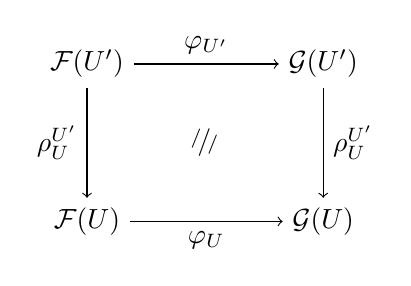
\begin{tikzpicture}[baseline=0]
  %Punkte definieren
  \node (a) at (-1.5,1){$\mathcal F(U')$};
  \node (b) at (1.5,1){$\mathcal G(U')$};
  \node (c) at (-1.5,-1){$\mathcal F(U)$};
  \node (d) at (1.5,-1){$\mathcal G(U)$};
  \node (0,0){$\schraffiert$};
  \draw[->] (a) -- node[above] {$\varphi_{U'}$} (b);
  \draw[->] (c) -- node[below] {$\varphi_U$} (d);
  \draw[->] (a) -- node[left] {$\rho_U^{U'}$} (c);
  \draw[->] (b) -- node[right] {$\rho_U^{U'}$} (d);
\end{tikzpicture} $\qquad$ f\"ur alle $U\subseteq U'$ in $\Off(X)$\end{center}
\end{Def}

\begin{DefBem}
Sei $\mathcal F$ eine Pr\"agarbe auf X.
\begin{enumerate}[a)]
\item
  F\"ur ein $x\in X$ sei
    \[\mathcal F_X = \lim_{x\in U \in \Off(X)} \mathcal F(U) = \FakRaum{\{(U,s): x\in U\in \Off(X), s\in \mathcal F(U)\}}{{\sim}}\]
  wobei $(U,s)\sim(U',s') :\Leftrightarrow \exists x\in U'' \subseteq U\cap U'$ mit $\rho_{U''}^U(s) = \rho_{U''}^{U'}(s')$
\item
  F\"ur $x\in U \in \Off(X)$ sei $\mathcal F(U) \to \mathcal F_X, s\mapsto (U,s)_{\sim} =: s_x$ der nat\"urliche Morphismus.
\item
  (UAE)\\
  F\"ur jedes $C\in \Ob \mathcal C$ und jede konsistente Familie $\varphi_U: \mathcal F(U) \to C$ von Morphismen in $\mathcal C$ gibt es genau einen Morphismus $\varphi_x: \mathcal F_X \to C$ mit $\varphi_x \circ \sigma_X = \varphi_U$ f\"ur alle $U$
    \[(U,s)_{\sim} \mapsto \varphi_U(s)\]
\item
  Jeder Morphismus $\varphi: \mathcal F \to \mathcal G$ induziert f\"ur jedes $x\in X$ einen Morphismus
    \[\varphi_x: \mathcal F_X \to \mathcal G_X\]
  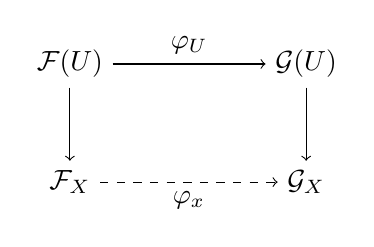
\begin{tikzpicture}
    \node (a) at (-1.5,1){$\mathcal F(U)$};
    \node (b) at (1.5,1){$\mathcal G(U)$};
    \node (c) at (-1.5,-0.5){$\mathcal F_X$};
    \node (d) at (1.5,-0.5){$\mathcal G_X$};

    \draw[->] (a) -- node[above] {$\varphi_{U}$} (b);
    \draw[->, dashed] (c) -- node[below] {$\varphi_x$} (d);
    \draw[->] (a) -- (c);
    \draw[->] (b) -- (d);
  \end{tikzpicture}
\end{enumerate}\end{DefBem}

%19. 4.

\begin{Bem}\label{1.7}
Sei $\calF$ Garbe von abelschen Gruppen auf $X$, $U\subseteq X$ offen, $s\in \calF(U)$.\\
Dann gilt:
  \[s=0 \Leftrightarrow s_x = 0 \text{ f\"ur alle } x\in U\]
\end{Bem}

\begin{bew}\begin{twosidedproof}
\proofforward
  $\checkmark$
\proofreverse
  F\"ur jedes $x\in U$ gibt es Umgebung $U_x$ mit $s|_{U_x} = 0$. ($s|_{U_x} = \rho_{U_x}^U$)\\
  Die $(U_x)_{x\in U}$ bilden offene \"Uberdeckungen, die $s|_{U_x}$ bilden konsistente Familie, $s$ und $0$ sind beides Amalgame $\xRightarrow[\text{eigenschaft}]{\text{Gruppen-}} s= 0$
\end{twosidedproof}\end{bew}

\begin{Prop}\label{1.8}
Seien $\calF, \calG$ Garben von abelschen Gruppen auf $X$, $\varphi: \calF \to \calG$ Morphismus.
\begin{enumerate}[a)]
\item\label{1.8a}
  $\varphi_U$ injektiv f\"ur jedes $U\in \Off(X) \Leftrightarrow \varphi_x$ injektiv f\"ur alle $x\in X$
\item
  $\varphi_U$ surjektiv f\"ur jedes $U\in \Off(X) \Rightarrow \varphi_x$ surjektiv f\"ur alle $x\in X$
\item
  $\varphi_U$ bijektiv f\"ur jedes $U\in \Off(X) \Leftrightarrow \varphi_x$ bijektiv f\"ur alle $x\in X$
\end{enumerate}\end{Prop}

\begin{bew}\begin{enumerate}[a)]
\item
  \begin{twosidedproof}
  \proofforward
    Sei $x\in X, s_x\in \calF$ mit $\varphi_x(s_x)=0$\\
    $\exists$ Umgebung von $x$ und $s\in \calF(U)$ mit $s_x =$ Keim von $s$ in $x$ mit $\varphi_x(s_x)=$ Keim von $\varphi_U(s)$ in $x = \varphi_U(s)_s$
    \begin{center}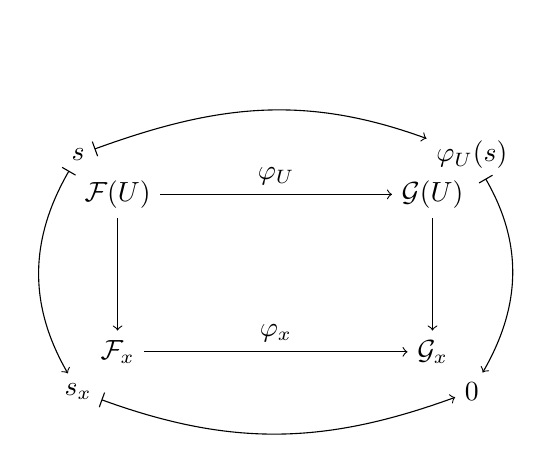
\begin{tikzpicture}
      \node (F) at (-2,1) {$\calF(U)$};
      \node (G) at (2,1) {$\calG(U)$};
      \node (Fx) at (-2,-1) {$\calF_x$};
      \node (Gx) at (2,-1) {$\calG_x$};
      
      \node (s) at (-2.5,1.5) {$s$};
      \node (phis) at (2.5,1.5) {$\varphi_U(s)$};
      \node (sx) at (-2.5,-1.5) {$s_x$};
      \node (0) at (2.5,-1.5) {$0$};
      
      \node (a) at (-0.5,3) {};
      
      \draw[->] (F) -- node[above] {$\varphi_{U}$} (G);
      \draw[->] (Fx) -- node[above] {$\varphi_{x}$} (Gx);
      \draw[->] (F) -- (Fx);
      \draw[->] (G) -- (Gx);
      
      \draw[|->] (s) to [out=20,in=160]  (phis);
      \draw[|->] (s) to [out=240,in=120] (sx);
      \draw[|->] (sx) to [out=340,in=200] (0);
      \draw[|->] (phis) to [out=300,in=60] (0);
    \end{tikzpicture}\end{center}
    $\Rightarrow$ \OE $\varphi_U(s) = 0 \underset{\varphi_U \text{ injektiv}}{\Longrightarrow} s= 0$
  \proofreverse
    Sei $U\subset \Off(X), s\in \calF(U)$ mit $\varphi_U(s) = 0$\\
    $\Rightarrow$ f\"ur alle $x\in U$ ist $\varphi_x(s_x) = \varphi_U(s)_x = 0 \xRightarrow{\varphi \text{ injektiv}} s_x = 0 \xRightarrow{\ref{1.7}} s = 0$
  \end{twosidedproof}
\item
  \begin{twosidedproof}
  \proofforward
    Sei $g_x\in\calG_x$, $(U,g)$ Repr\"asentant\\
    $\Rightarrow \exists s\in \calF(U)$ mit $\varphi_U(s)=g \Rightarrow \varphi_x(s_x) = g$
    \begin{center}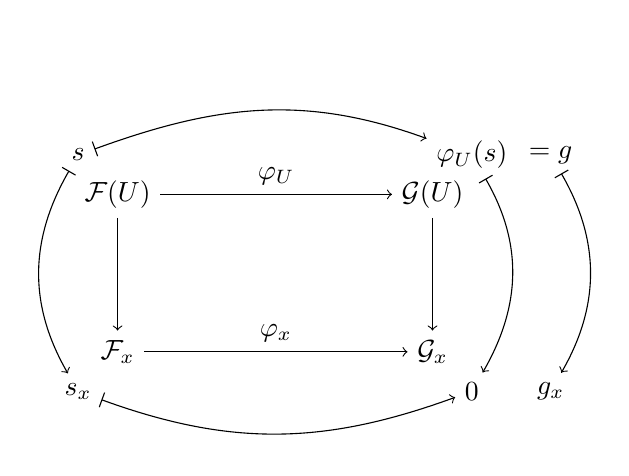
\begin{tikzpicture}
      \node (F) at (-2,1) {$\calF(U)$};
      \node (G) at (2,1) {$\calG(U)$};
      \node (Fx) at (-2,-1) {$\calF_x$};
      \node (Gx) at (2,-1) {$\calG_x$};
      
      \node (s) at (-2.5,1.5) {$s$};
      \node (phis) at (2.5,1.5) {$\varphi_U(s)$};
      \node (g) at (3.5,1.5) {$= g$};
      \node (sx) at (-2.5,-1.5) {$s_x$};
      \node (0) at (2.5,-1.5) {$0$};
      \node (gx) at (3.5,-1.5) {$g_x$};
      
      \node (a) at (-0.5,3) {};
      
      \draw[->] (F) -- node[above] {$\varphi_{U}$} (G);
      \draw[->] (Fx) -- node[above] {$\varphi_{x}$} (Gx);
      \draw[->] (F) -- (Fx);
      \draw[->] (G) -- (Gx);
      
      \draw[|->] (s) to [out=20,in=160]  (phis);
      \draw[|->] (s) to [out=240,in=120] (sx);
      \draw[|->] (sx) to [out=340,in=200] (0);
      \draw[|->] (phis) to [out=300,in=60] (0);
      \draw[|->] (g) to [out=300,in=60] (gx);
    \end{tikzpicture}\end{center}
  \end{twosidedproof}
  \begin{bsp}
  Sei $X = \C$, $\calO$ die Garbe der holomorphen Funktionen auf $\C$, $\calO^\X$ die Garbe der invertierbaren holomorphen Funktionen.\\
  $\varphi = \exp$, das hei\ss t f\"ur $f\in \calO(U)$ sei $\varphi(f) = e^{2\pi if}$.\\
  $\varphi$ ist Garbenhomomorphisms ($e^{f+g} = e^f \cdot e^g$). $\varphi_x$ ist surjektiv f\"ur jedes $x\in X$ (lokal gibt es zu jeder holomorphen Funktion ohne Nullstellen einen Logarithmus). $\varphi_{\C\setminus\{0\}}$ ist nicht surjektiv! (zum Beispiel gibt es keine holomorphe Funktion $\log z$ auf ganz $\C$)\\
  Schlimmer noch: $\varphi_U$ ist nicht injektiv f\"ur jedes $U \in \Off(\C)$, das nicht einfach zusammenh\"angend ist.
  \end{bsp}
\item
  \begin{twosidedproof}
  \proofforward
    $\checkmark$
  \proofreverse
    Sei $U\subseteq X$ offen, $g\in \calG(U)$.\\
    F\"ur jedes $x\in U$ gibt es $s_x\in \calF_x$ mit $\varphi_x(s_x) = g_x$.\\
    W\"ahle Repr\"asentanten $(U_x, s^{(x)})$ von $s_x$, sodass $\varphi_{U_x}(s^{(x)}) = g|_{U_x}$ (das geht!) (\emph{denn}: Sei $(U,\tilde s)$ Repr\"asentant von $s_x \Rightarrow \varphi_U(\tilde s)\sim_x g|_U \Rightarrow \exists x \in U_x \subset U: \varphi_U(\tilde s)|_{U_x} = g|_{U_x}$)\\
    Die $U_x$ bilden offene \"Uberdeckungen von $U$, die $s^{(x)}$ bilden konsistente Familie (*) $\Rightarrow \exists$ Amalgam $s\in \calF(U)$ mit $\varphi_U(s)|_{U_x} = \varphi_{U_x}(s^{(x)}) = g|_{U_x} \Rightarrow \varphi_U(s) = g$\\
    (*) zu zeigen: $s^{(x)}|_{U_x\cap U_y} = s^{(y)}|_{U_x\cap U_y}$\begin{description}[\setlabelstyle{\itshape}]
    \item[denn:] $\varphi_{U_x\cap U_y}(s^{(x)}|_{U_x\cap U_y} = \varphi_{U_x\cap U_y}(s^{(y)}|_{U_x\cap U_y}$, $\varphi_{U_x\cap U_y}$ injektiv nach Voraussetzung und a) $\Rightarrow $ Behauptung
    \end{description}
  \end{twosidedproof}
\end{enumerate}\end{bew}

\begin{PropDef}
Sei $X$ topoloischer Raum, $\calF$ Pr\"agarbe auf $X$ (mit Werten in $\calC$)
\begin{enumerate}[a)]
\item
  Es gibt genau eine Garbe $\calF^+$ auf $X$ und einen Morphismus $\vartheta: \calF \to \calF^+$, sodass $\vartheta_x:\calF_x \to \calF_x^+$ f\"ur jedes $x\in X$ ein Isomorphismus ist.
\item
  $\calF^+$ hei\ss t \deftermspec{zu $\calF$ assoziierte Garbe}{Garbe!assoziierte}.
\item(UAE)\\
  F\"ur jeden Morphismus $\varphi: \calF \to \calG$ in eine Garbe $\calG$ gibt es genau einen Morphismus $\varphi^+: \calF^+ \to \calG$ mit $\varphi = \varphi^+ \circ \vartheta$.
  \begin{center}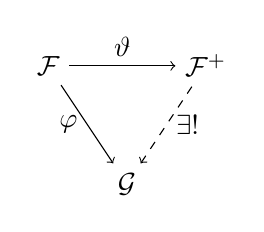
\begin{tikzpicture}
    \node (F) at (-1,0) {$\calF$};
    \node (F+) at (1,0) {$\calF^+$};
    \node (G) at (0,-1.5) {$\calG$};
    
    \draw[->] (F) -- node[above]{$\vartheta$} (F+);
    \draw[->] (F) -- node[left]{$\varphi$} (G);
    \draw[->, dashed] (F+) -- node[right]{$\exists!$} (G);
  \end{tikzpicture}\end{center}
\end{enumerate}\end{PropDef}

\begin{bew}\begin{enumerate}[a)]\item
F\"ur $U\in \Off(X)$ sei
  \[\begin{array}{rcl}\calF^+(U) &:=& \{s: U\to \dot{\bigcup\limits_{x\in U}}\calF_x | s(x)\in \calF_x \forall x\in X \text{, zu jedem } x\in U \\ &&\text{ gibt es Umgebung } U_x \text{ und } f\in \calF(U) \text{ mit } s(y) = f_y \\&& \text{ f\"ur jedes } y \in U_y\}\end{array}\]
$\calF^+$ ist Garbe $\checkmark$\\
Sei $\vartheta: \calF \to \calF^+$ gegeben durch
  \[\boxed{\vartheta_U(f)(x) = f_x \quad (U\in \Off(X), f\in \calF(U))}\]
$\vartheta$ ist Morphismus: $\checkmark$\\
$\vartheta$ ist Isomorphismus: $\checkmark$
\end{enumerate}\end{bew}

\begin{DefBem}
Sei $\varphi:\calF \to \calG$ Morphismus von Garben abelscher Gruppen auf $X$.
\begin{enumerate}[a)]
\item
  Sei $\Kern(\varphi)$ die Pr\"agarbe $\Kern(\varphi)(U) := \Kern(\varphi_U)$.
\item
  $\Kern(\varphi)$ ist Garbe.
\item
  $\varphi$ hei\ss t \defterm{injektiv} (oder \defterm{Monomorphismus}) $:\Leftrightarrow \Kern(\varphi) = 0$
    \[\begin{array}{c}\mathcal E_1\overset{\psi_1}{\to}\\\mathcal E_2\overset{\psi_2}{\to}\end{array}\calF \overset{\varphi}{\to} \calG\]
  $\varphi$ Monomorphismus $\Leftrightarrow \varphi \circ \psi_1 = \varphi \circ \psi_2 \Rightarrow \psi_1  = \psi_2$
\item
  Sei $\calB_\varphi$ die Pr\"agarbe $\calB_\varphi(U) := \Bild(\varphi_U)$\\
  $\Bild(\varphi_U) := \calB_\varphi^+$
\item
  $\varphi$ hei\ss t \defterm{surjektiv} (oder \defterm{Epimorphismus}) $:\Leftrightarrow \Bild(\varphi) = \calG$
      \[\calF \overset{\varphi}{\to} \calG \begin{array}{c}\overset{\psi_1}{\to}\mathcal H_1\\\overset{\psi_2}{\to}\mathcal H_2\end{array}\]
  $\varphi$ Epimorphismus $\Leftrightarrow \psi_1 \circ \varphi = \psi_2 \circ \varphi \Rightarrow \psi_1 = \psi_2$
\end{enumerate}\end{DefBem}

\begin{bew}\begin{enumerate}[a)]
\item \textcolor{white}{a} %<-- ohne das wird das Design zerschossen
  \begin{center}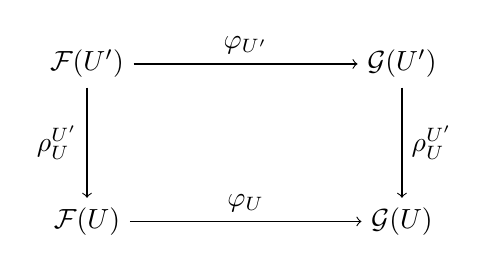
\begin{tikzpicture}
    \node (FU') at (-2,1) {$\calF(U')$};
    \node (GU') at (2,1) {$\calG(U')$};
    \node (FU) at (-2,-1) {$\calF(U)$};
    \node (GU) at (2,-1) {$\calG(U)$};
    
    \draw[->] (FU') --node[above]{$\varphi_{U'}$} (GU');
    \draw[->] (FU') --node[left]{$\rho_{U}^{U'}$} (FU);
    \draw[->] (GU') --node[right]{$\rho_{U}^{U'}$} (GU);
    \draw[->] (FU) --node[above]{$\varphi_{U}$} (GU);
  \end{tikzpicture}\end{center}
\item
  Sei $(U_i)_{i\in I}$ offene \"Uberdeckung von $U\in \Off(X)$, $s_i \in \Kern(\varphi_{U_i}) \subseteq \calF(U_i)$ konsistente Familie.\\
  $\exists!$ Amalgam $s\in \calF(U)$.\\
  $\varphi_x(s_x) = 0$ f\"ur jedes $x\in U$ $\xRightarrow{\ref{1.8} \ref{1.8a})} \varphi_U(s) = 0$
%25.4.
\item[e)]
  $\Bild(\varphi) = \calG \Leftrightarrow \underbrace{\Bild(\varphi)_x}_{=\Bild(\varphi_x)} = \calG_x$ f\"ur alle $x$\\
  $\varphi$ Epimorphismus $\Leftrightarrow$ f\"ur jedes $x\in X$ ist $\varphi_x$ surjektiv, das hei\ss t $\Bild(\varphi_x) = \calG_x$.
\end{enumerate}\end{bew}

\begin{Def}
Seien $\calF, \calG$ Garben abelscher Gruppen auf $X$, $i:\calG \to \calF$ Monomorphismus.
\begin{enumerate}[a)]
\item
  $\calG$ hei\ss t \defterm{Untergarbe}\index{Garbe!Unter} von $\calF$.
\item
  $U\mapsto \FakRaum{\calF(U)}{\calG(U)}$ ist Pr\"agarbe auf $X$, die assoziierte Garbe $\FakRaum{\calF}{\calG}$ hei\ss t \defterm{Quotientengarbe}\index{Garbe!Quotienten}.
\end{enumerate}\end{Def}

\begin{bsp}
\begin{minipage}[t]{0.6\textwidth}
Sei $X=S^1$ (Einheitskreislinie)\\
$\calF = \calC$ (stetige Funktionen $S^1\to \R$)\\
$\calG = $ konstante Garbe $\Z$\\
$U = x$, $U_1, U_2$ wie im Bild
\end{minipage}
\begin{minipage}[t]{0.4\textwidth}
\textcolor{white}{[ ! BILD ! ]}\\
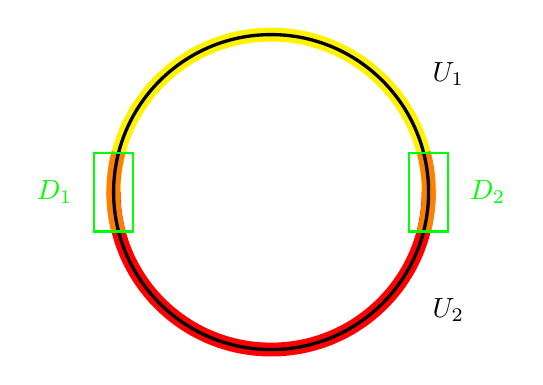
\begin{tikzpicture}
  \node at (-2.75,0) {\textcolor{green}{$D_1$}};
  \node at (2.75,0) {\textcolor{green}{$D_2$}};
  
  \node at (2.25,1.5) {$U_1$};
  \node at (2.25,-1.5) {$U_2$};
  
  \draw[yellow, line width=5] (2,0) arc (0:180:2);
  \draw[red, line width=5] (-2,0) arc (180:360:2);
  
  \draw[orange, line width=5] (-1.94,0.5) arc (165.5:194.5:2);
  \draw[orange, line width=5] (1.94,-0.5) arc (-14.5:14.5:2);
  
  \draw[very thick] (0,0) circle (2);

  \draw[green, thick] (-2.25,0.5) -- (-2.25,-0.5) -- (-1.75,-0.5) -- (-1.75,0.5) -- cycle;
  \draw[green, thick] (2.25,0.5) -- (2.25,-0.5) -- (1.75,-0.5) -- (1.75,0.5) -- cycle;
\end{tikzpicture}
\end{minipage}
  \[U_1 \cap U_2 = D_1 \cup D_2\]
Sei $f_1 \in \calF(U_1)$ mit $f_1|_{D_1} = 0, f_1|_{D_2} = 1, 0 = f_2 \in \calF(U_2)$\\
$\Rightarrow f_1|_{U_1\cap U_2} \in \calG(U_1\cap U_2)$ (!)\\
$\bar{f_1} = \bar{f_2}$ in $\FakRaum{\calF(U_1\cap U_2)}{\calG(U_1\cap U_2)}$\\
$\Rightarrow (\bar{f_i} \in \FakRaum{\calF(U_i)}{\calG(U_i)})_{i=1,2}$ ist konsistente Familie.\\
\emph{Aber:} Es gibt kein $f\in \calF(U)$ mit $f|_{U_1} = f_1, f|_{U_2} = f_2$
\end{bsp}

\begin{Prop}
Sei $X$ topologischer Raum, $U\subseteq X$ offen, $x\in X$.
\begin{enumerate}[a)]
\item
  Die Zuordnung $\Phi: \calF \mapsto \calF_x$ induziert exakten kovarianten Funktor von der Kategorie $\Sh(X)$ der Garben abelscher Gruppen auf $X$ in die Kategorie $\Ab$ der abelschen Gruppen.\\
  Dabei ist $\Phi_x(\varphi) = \varphi_x$ f\"ur $\varphi: \calF \to \calG$ Morphismus.
\item
  Die Zuordnung $\Phi_U: \F \to \F(U)$ induziert linksexakten kovarianten Funktor $\Sh(X) \to \Ab$ (mit $\Phi_U(\varphi) = \varphi_U$)
\end{enumerate}\end{Prop}

\begin{bew}
(*) Sei $0 \to \F' \overset{\varphi}{\to} \F \overset{\psi}{\to} \F'' \to 0$ exakte Sequenz in $\Sh(X)$. \textbf{Achtung:} Das bedeutet \emph{nicht}, dass f\"ur jedes $\widetilde U \in \Off(X)$ die Sequenz $0 \to \F'(\widetilde U) \to \F(\widetilde U) \to \F''(\widetilde U) \to 0$ exakt sein muss.\\
Aber: (*) ist \"aquivalent zu: $0 \to \F'_y \overset{\varphi_y}{\to} \F_y \overset{\psi_y}{\to} \F''_y \to 0$ ist exakt f\"ur jedes $y \in X$\\
$\Rightarrow $ a)
\begin{enumerate}[a)]\item[b)]
$\Phi_U$ linksexakt bedeutet:
  \[0 \to \F'(U) \overset{\varphi_U}{\to} \F(U) \overset{\psi_U}{\to} \F''(U) \to 0 \text{ ist exakt}\]
Das stimmt nach \ref{1.8} und \dots
\end{enumerate}\end{bew}

\begin{DefBem}
Sei $f: X\to Y$ stetig.
\begin{enumerate}[a)]
\item
  Sei $\F$ Garbe auf $X$.\\
  Dann ist die Pr\"agarbe $U\mapsto \F(f^{-1}(U))$ auf $Y$ eine Garbe, sie hei\ss t (direkte) \defterm{Bildgarbe}\index{Garbe!Bild} von $\F$ (unter $f$). Bezeichnung: $f_*\F$
\item
  Sei $\G$ Garbe auf $Y$.\\
  Die zur Pr\"agarbe $U\mapsto \lim\limits_{\substack{f(U)\subseteq V\\ V\in \Off(Y)}} \G(V)$ assoziierte Garbe hei\ss t \defterm{Urbildgarbe}\index{Garbe!Urbild} von $\G$.\\
  Bezeichnung: $f^{-1}(G)$
\item
  $f_*$ und $f^{-1}$ sind kovariante Funktoren.
\end{enumerate}\end{DefBem}

\begin{bew}\begin{enumerate}[a)]
\item
  Sei $U\subseteq Y$ offen, $(U_i)_{i\in I}$ offene \"Uberdeckung von $U$, also $(f^{-1}(U_i))_{i\in I}$ offene \"Uberdeckung von $f^{-1}(U)$. $s_i \in \underbrace{f_*\F(U_i)}_{=\F(f^{-1}(U_i))}$, $i \in I$, konsistente Familie.\\
  $\Rightarrow \exists$ Amalgam $s\in \underbrace{\F(f^{-1}(U))}_{=f_*\F(U)}$ mit $s|_{f^{-1}(U_i)} = s_i$ f\"ur alle $i \in I$.
\item[c)]
  Sei $\varphi:\F \to \G$ Morphismus von Garben auf $X$.
  \begin{enumerate}[i)]
  \item
    Definiere $\varphi_*: f_*\F \to f_* \G$ durch
      \[(\varphi_*)_U = \varphi_{f^{-1}(U)}: f_*\F(U) = \F(f^{-1}(U)) \to f_x\G(U) = \G(f^{-1}(U))\]
  \item
    Definiere $f^{-1}\varphi: f^{-1}\F \to f^{-1}\G$ durch $(f^{-1}_\varphi)_U = \lim\limits_{f^{-1}(U)\subseteq V\in \Off(Y)} \varphi_V$\\
    \begin{center}$V'\subseteq V \qquad$
    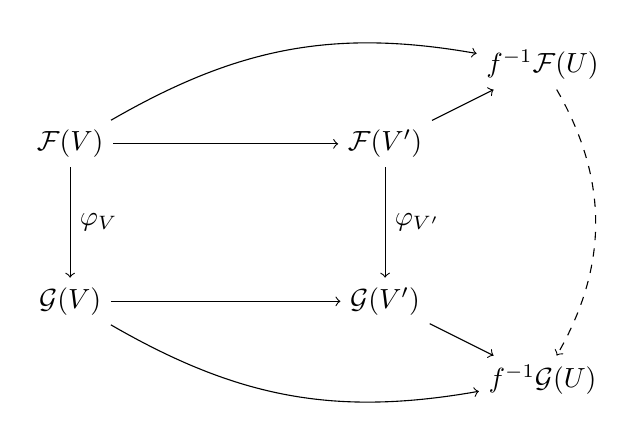
\begin{tikzpicture}[baseline = 0]
      \node (FV) at (-2,1) {$\F(V)$};
      \node (FV') at (2,1) {$\F(V')$};
      \node (GV) at (-2,-1) {$\G(V)$};
      \node (GV') at (2,-1) {$\G(V')$};
      
      \node(fF) at (4,2) {$f^{-1}\F(U)$};
      \node(fG) at (4,-2) {$f^{-1}\G(U)$};
      
      \draw[->] (FV) -- (FV');
      \draw[->] (FV) -- node[right]{$\varphi_V$} (GV);
      \draw[->] (GV) -- (GV');
      \draw[->] (FV') -- node[right]{$\varphi_{V'}$} (GV');
      
      \draw[->] (FV) to [out=30,in=170] (fF);
      \draw[->] (GV) to [out=330,in=190] (fG);
      \draw[->] (FV') -- (fF);
      \draw[->] (GV') -- (fG);
      \draw[->, dashed] (fF) to [out=300,in=60] (fG);
    \end{tikzpicture}\end{center}
  \end{enumerate}
\end{enumerate}\end{bew}

\begin{Prop}
Sei $f:X\to Y$ stetig, $\F$ eine Garbe auf $X$, $\G$ Garbe auf $Y$.\\
Dann gibt es eine (nat\"urliche) Bijektion
  \[\Hom(f^{-1}\G, \F) \to \Hom(\G, f_*\F)\]
Das bedeutet: $f^{-1}$ ist linksadjungiert zu $f_*$.
\end{Prop}

\begin{bew}
Definiere $\varphi_\F: f^{-1}f_*\F \to \F$ und $\psi_\G: \G \to f_*f^{-1}\F$\\
Dann:
  \[ T_1:\left\{ \begin{array}{ccc}\Hom(f^{-1}\G,\F) &\to& \Hom(\G, f_*\F)\\
  \alpha &\mapsto& f_*(\alpha)\circ\psi_\G: \G \to f_*f^{-1}\G \overset{f_*\alpha}{\to} f_*\F\end{array}\right.\]
Analog: $T_2: \beta \mapsto \varphi_\F \circ f^{-1}(\beta)$\\
Rest: \"Ubung
\end{bew}

\newpage
%-------------------------- Abschnitt 2 (Affine Schemata) --------------------------
%26. 4.

\section{Affine Schemata}

\begin{description}
\item[Behauptung:]
  $\alpha:R\to R'$ Ringhomom., $\p\subset R'$ Primideal $\Rightarrow \alpha^{-1}(\p)$ Primideal in $R$
\item[Beweis:]
  Seien $f,g \in R$ mit $f\cdot g \in \alpha^{-1}(\p)$\\
  $\Rightarrow \underbrace{\alpha(f\cdot g)}_{=\alpha(f)\cdot\alpha(g)} \in \p \xRightarrow{\text{\OE}} \alpha(f) \in \p \Rightarrow f \in \alpha^{-1}(\p)$
\end{description}

\begin{DefBem}
Sei $R$ ein Ring (das hei\ss t kommutativer Ring mit Eins)
\begin{enumerate}[a)]
\item
  $\Spec R:= \{\p \subset R: \p \text{ Primideal}\}$ hei\ss t \defterm{Spektrum} von $R$.
\item
  F\"ur $I\subseteq R$ sei $V(I)=\{\p \in \Spec R: I \subseteq \p\}$. $V(I)$ hei\ss t \defterm{Nullstellenmenge} (vanishing set) von $I$, es ist $V(I) = V((I))$.
\item
  Die $V(I)$, $I\subseteq R$ Ideal, bilden die abgeschlossenen Mengen einer Topologie auf $\Spec R$, der \defterm{Zariski-Topologie}.
\item
  F\"ur $V\subseteq \Spec R$ hei\ss t $I(V):= \bigcap\limits_{\p \in V}\p$ \defterm{Verschwindungsideal} von $V$.
\end{enumerate}\end{DefBem}

\begin{bew}\begin{enumerate}[a)]\item[c)]
$\emptyset = V(R)$\\
$\Spec R = V(0)$\\
$\bigcap\limits_{i\in I} V(I_i) = \bigcap\limits_{i\in I}\{\p \in I_i \subseteq \p\} = \{\p: I_i \subseteq \p \forall i\} = V(\bigcup\limits_{i\in I} I_i) = V(\sum\limits_{i\in I} I_i)$\\
$V(I_1)\cup V(I_2) = \{\p \in \Spec R: I_1 \subseteq \p \text{ oder } I_2 \subseteq \p\} = V(I_1\cdot I_2) \overset{?}{=} V(I_1\cap I_2)$\\
\hspace*{10mm} $I_1\cdot I_2 \subseteq I_1 \cap I_2 \Rightarrow V(I_1\cdot I_2) \supseteq V(I_1\cap I_2)$\\
\hspace*{10mm} $\p \in V(I_1\cdot I_2) \Rightarrow I_1\cdot I_2 \subseteq \p \xRightarrow{\text{\OE}} I_1 \subseteq \p \Rightarrow I_1\cap I_2 \subseteq \p$\\
$\Rightarrow V(I_1\cdot I_2) = V(I_1\cap I_2)$
\end{enumerate}\end{bew}

\begin{Bem}\begin{enumerate}[a)]
\item
  $V(I(V)) = \bar{V}$ f\"ur jedes $V\subseteq \Spec R$
\item
  $I(V(I)) = \sqrt{I}$ f\"ur jedes ideal $I\subseteq R$
\end{enumerate}\end{Bem}

\begin{bew}\begin{enumerate}[a)]
\item
  \begin{twosidedproof}
  \proofsupseteq
    $V\subseteq V(I(V)) = \{\q \in \Spec R: \bigcap\limits_{\p \in V} \p \subseteq \q \}$
  \proofsubseteq
    Es ist $\bar{V} = \bigcap\limits_{V\subseteq V(I)}V(I)$\\
    Ist $I$ Ideal in $R$ mit $V\subseteq V(I)$, so ist $I\subseteq I(V) = \bigcap\limits_{\p \in V} \p$.\\
    $\Rightarrow V(I) \supseteq V(I(V))$\\
    $\Rightarrow V(I(V)) \subseteq \bigcap\limits_{I:V\subseteq V(I)} V(I) = \bar{V}$
  \end{twosidedproof}
\item
  $I(V(I)) = \bigcap\limits_{\p \in V(I)} \p = \bigcap\limits_{I\subseteq \p} \p \overset{!}{=} \sqrt{I}$ (\"Ubung)
\end{enumerate}\end{bew}

\begin{Prop}
Sei $V\subseteq \Spec R$ abgeschlossen, $V\ne 0$.\\
Dann gilt: $V$ irreduzibel $\Leftrightarrow I(V)$ Primideal
\end{Prop}

\begin{bew}
Wie in Algebraische Geometrie I, Proposition 4.4
\end{bew}

\begin{Bem}\label{2.4}
Jeder Ringhomomorphismus $\alpha: R \to R'$ induziert stetige Abbildung $f_\alpha:\Spec R' \to R$ durch $\p \mapsto \alpha^{-1}(\p)$, das hei\ss t $\Spec: \left\{\begin{array}{ccc} \Ringe &\to& \Top \\ R &\mapsto& \Spec R\end{array}\right.$ ist kontravarianter Funktor.
\end{Bem}

\begin{bew}
Noch zu zeigen: $f_\alpha$ stetig\\
Sei $V=V(I) \subseteq \Spec R$\\
$\Rightarrow f_\alpha^{-1}(V) = \{\p \in \Spec R': \alpha^{-1}(\p) \supseteq I\} = \{ \p: \p \supseteq \alpha(I)\} = V(\alpha(I))$
\end{bew}

\begin{Bem}
Sei $k$ algebraisch abgeschlossener K\"orper, $V\subseteq \A^n(k)$ affine Variet\"at.\\
Dann ist $m: \left\{ \begin{array}{ccc} V &\to& \Spec k[V]\\ x &\mapsto& m_x\end{array}\right.$ injektiv und stetig.
\end{Bem}

\begin{bew}
injektiv: $\checkmark$\\
$m$ stetig: Sei$V(I) \subseteq \Spec k[V]$ abgeschlossen.\\
$\Rightarrow m^{-1}(V(I)) = \{ x\in V: m_x \in V(I)\} = \{x: I \subseteq m_x\} = \{x: f(x) = 0$ f\"ur alle $f\in I\} = V(I)$
\end{bew}

\begin{bsp}
Seien $\p \subsetneq\q$. Dann ist $\q \in \overline{\{\p\}}$
\end{bsp}

\begin{DefBem}\begin{enumerate}[a)]
\item
  Ein Punkt $x\in X$ ($X$ topologischer Raum) hei\ss t \defterm{generisch}, wenn $\overline{\{x\}} = X$ ist.
\item
  Jede irreduzible Teilmenge von $\Spec R$ hat genau einen generischen Punkt.
\item
  Die irreduziblen Komponenten von $\Spec R$ entsprechen bijektiv den minimalen Primidealen in $R$.
\end{enumerate}\end{DefBem}

\begin{Bem}
F\"ur jedes $f\in R$ ist $D(f) = \Spec R\setminus V(f) = \{\p \in \Spec R : f \notin \p\}$ offen in $\Spec R$. Die $D(f), f\in R$ bilden eine Basis der Zariski-Topologie.
\end{Bem}

\begin{bew}
Sei $U\subseteq \Spec R$ offen, $V= \Spec R - U \Rightarrow \exists I \subseteq R$ Ideal mit $V=V(I)$\\
F\"ur $f\in I$ ist $f\in \p$ f\"ur jedes $\p \in V$, das hei\ss t $V(I) \subseteq V(f) \Rightarrow D(f) \subseteq U$
\end{bew}

\begin{Bem}
$\Spec R$ ist quasikompakt.
\end{Bem}

\begin{bew}
Sei $(U_i)_{i\in I}$ offene \"Uberdeckung von $\Spec R$.\\
\OE $U_i = D(f_i)$ f\"ur ein $f_i\in R$\\
Dann gilt : $\bigcup\limits_{i\in I}D(f_i) = \Spec R \Leftrightarrow\bigcap\limits_{i\in I}V(f_i) = \emptyset \Leftrightarrow$ Die $f_i$, $i \in I$, erzeugen $R$\\
$\Rightarrow \exists i_1,\ldots ,i_k$ mit $1=\sum\limits_{\nu=1}^k a_\nu f_{i_\nu}$ f\"ur gewisse $a_\nu \in R$\\
$\Rightarrow \bigcup\limits_{\nu = 1}^k D(f_{i_\nu}) = \Spec R$
\end{bew}

%2.5.
\begin{DefBem}
Sei $R$ ein Ring, $X = \Spec R$
\begin{enumerate}[a)]
\item
  F\"ur $f \in R$ sei $\calO_X(D(f)) := R_f$
\item
  Die Zuordnung $D(f) \mapsto R_f$ ist eine $\calB$-Garbe von Ringen auf $X$ f\"ur die Basis $\calB = \{D(f): f\in R\}$ der Zariski-Topologie auf $X$.
\item
  Es gibt eine eindeutig bestimmte Garbe $\calO_X$ von Ringen auf $X$ mit $\calO_X(D(f)) = R_f$ f\"ur jedes $f\in R$.\\
  $\calO_X$ hei\ss t \defterm{Strukturgarbe}\index{Garbe!Struktur-} auf $X$.
\item
  F\"ur beliebiges $U\subseteq X$ offen ist $\calO_X(U) = \{ s: U \to \bigsqcup\limits_{\p\in U}^{\cdot} R_\p \vert s(\p) \in R_\p$ f\"ur alle $\p \in U$; f\"ur jedes $\p \in U$ gibt es Umgebung $U_\p \subseteq U$ von $\p$ und $f,g \in R$ mit $g\notin \q$ f\"ur alle $\q \in U_\p$ sodass $s(\q) = \frac{f}{g}(\q)$ f\"ur alle $\q \in U_\p\}$\\
  \textcolor{gray}{$g\notin \q$ bedeutet $\q \in D(g)$; $\frac{f}{g}(\q) := \Bild$ von $\frac{f}{g}$ in $R_\q$}
\item
  $\calO_{X,\p} \cong R_\p$ f\"ur jedes $\p \in X$.
\end{enumerate}\end{DefBem}

\begin{bew}\begin{enumerate}[a)]\item[b)]
Seien $f,g \in R$ mit $D(f) \subseteq D(g)$.\\
$\Rightarrow V(g) \subseteq V(f) \Rightarrow f\in \bigcap\limits_{(g)\in \p} \p = \sqrt{(g)}$\\
$\Rightarrow \exists d \ge 1$ mit $f^d \in (g)$, das hei\ss t $\exists h \in R$ mit $f^d = g\cdot h$\\
$\Rightarrow $ erhalte Homomorphismus $\begin{array}{ccc} R_g &\to& R_f \\ \frac{a}{g^k} &\mapsto& \frac{a\cdot h^k}{f^{d\cdot k}}\end{array}$\\
\emph{Wohldefiniertheit:} $\frac{g}{1} \cdot \frac{h}{f^d} = 1$ in $R_f$, da $g\cdot h - f^d = 0$ in $R_f$.\\
\emph{Zeige:} $D(f) \mapsto R_f$ ist $\calB$-Garbe.\\
Sei also $f\in R$, $(D(f_i))_{i\in I}$ offene \"Uberdeckung von $D(f)$, $g_i \in R_{f_i}$ konsistente Familie (das hei\ss t $g_i = g_j$ in $\calO_X(D(f_i) \cap D(f_j)) = \calO(D(f_if_j)) = R_{f_if_j}$).\\
\emph{Zu zeigen:} $\exists! g \in R_f$ mit $g = g_i$ in $R_{f_i}$ f\"ur jedes $i$:\begin{description}[\setlabelstyle{\itshape}]
\item[$\bullet$]
  \OE $f = 1$, $I=\{1,\ldots ,n\}$ ($X$ ist quasikompakt)
\item[$\bullet$ Eindeutigkeit:]
  Ist $g=h$ in $R_{f_i}$, $i=1,\ldots ,n$, so ist $(g-h)\cdot f_i^d = 0$ f\"ur ein $d\ge 1$. Die $f_i^d$, $i=1,\ldots ,n$, erzeugen $R$ (!)
    \[(f_1,\ldots ,f_n)^{n\cdot d} \subseteq (f_1^d,\ldots ,f_n^d)\]
  $\Rightarrow g = h$
\item[$\bullet$ Existenz:]
  Schreibe $g_i = \frac{h_i}{f_i^N}$, $h_i \in R$, $N\ge 1$. Nach Voraussetzung ist $\overbrace{f_i^Nf_j^Ng_i}^{=f_j^Nh_i} = \overbrace{f_j^Nf_i^Ng_j}^{f_i^Nh_j}$ f\"ur ein (anderes) $N\ge 1$.\\
  $(f_1^N,\ldots ,f_n^N) =R \Rightarrow \exists b_i \in R$ mit $ 1 = \sum\limits_{i=1}^n b_if_i^N$\\
  Setze $g:= \sum\limits_{i=1}^n b_ih_i$\\
  Dann ist f\"ur $j=1,\ldots ,n$
    \[f_j^Ng = f_j \sum\limits_{i=1}^n b_ih_i = \sum\limits_{i=1}^n b_if_j^Nh_i = \underbrace{\sum\limits_{i=1}^n b_if_i^N}_{=1}h_j = h_j = f_j^Ng_j \text{ in } R_{f_j}\]
  $\Rightarrow g= g_j$ in $R_{f_j}$
\end{description}\end{enumerate}\end{bew}

\begin{Def}
Sei $R$ ein Ring, $X = \Spec R$, $\calO_X$ die Strukturgarbe.\\
Dann hei\ss t $(X,\calO_X)$ \defterm{affines Schema}\index{Schema!affines}.
\end{Def}

\begin{bspe}\begin{enumerate}[1)]
\item
  $R=k$ K\"orper $\Rightarrow X= \Spec k = \{(0)\}$, $\calO_X(X) = k$
\item
  $R= k[X], k$ K\"orper. Ist $\{(0)\}$ offen? Nein!\\
  $k = \Q$: $\p = (X^2+X+1)$ ist abgeschlossener Punkt
    \[\FakRaum{R_\p}{m_\p} \cong \FakRaum{\Q[X]}{(X^2+X+1)} = \Q(\zeta_3)\]
  $\Rightarrow \q = (X-a), a\in k$, $\FakRaum{R_\q}{m_\q} \cong \FakRaum{k[X]}{(X-a)} \cong k$
\end{enumerate}\end{bspe}

\begin{Bem}\label{2.11}
Sei $(X,\calO_X)$ affines Schema, $X= \Spec R$.\\
Dann ist f\"ur jedes $f\in R$ auch $(D(f), \calO_X(f))$ affines Schema. \emph{Genauer:} $(D(f), \calO_X(D(f))) = (\Spec R_f, \calO_{\Spec R_f})$
\end{Bem}

\begin{bew}
$D(f) = \{ \p \subset R \text{ Primideal}: f\notin R\}$\\
$\Spec R_f = \{\p \subset R \text{ Primideal}\}$
  \[\begin{array}{ccc} R &\to& R_f \\ a &\mapsto& \frac{a}{1}\end{array}\]
$\p \subsetneq \q \not\ni f$, $\p \cdot R_f = \q \cdot R_f$\\
Sei $x \in \q\setminus \p \overset{!}{\Rightarrow} \frac{x}{1} \notin \p \cdot R_f$\\
Sei $x= \frac{a}{f^d}, a \in \p, d\ge 1 \Rightarrow f^d \cdot x \in \p \lightning$\\
Sei $h = \frac{g}{f^d} \in R_f$. \emph{Zu zeigen:}
  \[ \underbrace{\calO_x|_{D(f)} (D(h))}_{\calO_X(D(f)\cap D(g) = R_{f\cdot g}} \cong \underbrace{\calO_{\Spec R_f}(D(h))}_{(R_f)_h = R_{f\cdot g}} \]
\end{bew}

\newpage
%-------------------------- Abschnitt 3 (Affine Schemata) --------------------------
%3. 5.

\section{(allgemeine) Schemata}

\begin{Def}\begin{enumerate}[a)]
\item
  Ein \defterm{geringter Raum} ist ein topologischer Raum $X$ zusammen mit einer Garbe $\calO_X$ von Ringen.
\item
  Ein geringter Raum $(X, \calO_X)$ hei\ss t \defterm{lokal}\index{geringter Raum!lokal} geringter Raum, wenn f\"ur jedes $x\in X$ der Halm $\calO_{X,x}$ ein lokaler Ring ist.
\end{enumerate}\end{Def}

\begin{Bem}
Jedes affine Schema $(\Spec R, \calO_{\Spec R})$ ist ein lokal geringter Raum.
\end{Bem}

\begin{Def}\label{3.3}\begin{enumerate}[a)]
\item
  Ein \defterm{Morphismus} $f:(X,\calO_X) \to (Y, \calO_Y)$ ist eine stetige Abbildung $f:X \to Y$ zusammen mit einem Morphismus $f^\#: \calO_Y \to f_*\calO_X$ von Garben.
\item\label{3.3b}
  Ein Morphismus zwischen lokal geringten R\"aumen $(X, \calO_X)$ und $(Y, \calO_Y)$ ist ein Morphismus $f: (X, \calO_X) \to (Y, \calO_Y)$ wie in a) sodass f\"ur jedes $x\in X$ der auf den Halmen induzierte Homomophismus $f_x^\#: \calO_{Y,f(x)} \to \calO_{X,x}$ die Bedingung $f_x^\#(m_{f(x)}) \subseteq m_x$ erf\"ullt ($f_x^\#$ hei\ss t dann lokaloer Homomophismus).\\
  $(f_* \calO_X)_{f(x)} = \lim\limits_{f(x) \in U} \calO_X(\underbrace{f^{-1}(U)}_{x\in}) \to \calO_{X,x}$
\end{enumerate}\end{Def}

\begin{bsp}
Sei $R$ lokaler Ring, nullteilerfrei, $K= \Quot(R) \ne R$. Dann ist die Inklusion $R \hookrightarrow K$ \emph{nicht} lokal.
\end{bsp}

\begin{Prop}\label{3.4}
Die Kategorie der affinen Schemata mit Morphismen aus Definition \ref{3.3} \ref{3.3b}) ist (anti-)\"aquivalent zur Kategorie der Ringe.
\end{Prop}

\begin{bew}\begin{enumerate}[(i)]\item
Sie Zuordnung $R\to (\Spec R, \calO_{\Spec R})$ ist Funktor. Sei $\alpha: R\to S$ Ringhomomorphismus, $f_\alpha: \Spec S \to \Spec R, \p \mapsto \alpha^{-1}(\q)$. Nach Bemerkung \ref{2.4} ist $f_\alpha$ stetig und $f_\alpha^{-1}(D(g)) = D(\alpha(g))$.

Definiere $f_\alpha^\# : \calO_{\Spec R} \to (f_\alpha)_* \calO_{\Spec S}$ durch
  \[\begin{array}{rcccr} \underbrace{\calO_{\Spec R}(D(g))} &\to& (f_\alpha)_* \calO_{\Spec S} (D(g)) =& \calO_{\Spec S} (f_\alpha^{-1}(D(g)) =& \underbrace{\calO_{Spec S} (D(\alpha(g))}\\
    = R_g \ni \frac{a}{g^d} &\mapsto& \frac{\alpha(a)}{\alpha(g)^d} &\in& =S_{\alpha(g)}\end{array}\]
\emph{Noch zu zeigen:} $(f_\alpha^\#)_\q$ ist lokal f\"ur jedes $\q\in \Spec S$

Sei $\p = \alpha^{-1}(\q) \in \Spec R$, das hei\ss t $\p = f_\alpha(\q)$.\\
Das maximale Ideal $m_\p$ (beziehungsweise $m_\q$) in $\calO_{\Spec R, \p} (=R_\p)$ (beziehungsweise $\calO_{\Spec S, \q}$) ist $\p R_\p$ (beziehungsweise $\q R_\q$).\\
F\"ur $a = \frac{b}{f} \in m_\p$ ($b \in \p, f\notin \p$) ist $(f_\alpha^\#)_\q(a) = \frac{\alpha(b)}{\alpha(f)} \in m_\q$, da $b\in \q = \alpha^{-1}(\q)$, also $\alpha(b) \in \q$ und $f\notin \p = \alpha^{-1}(\q)$, also $\alpha(f) \notin \q$.
\end{enumerate}\end{bew}

\begin{bsp}[Fortsetzung des Beispiels]
$\alpha: R\hookrightarrow K$, $\dim R = 1$ (zum Beispiel diskreter Bewertungsring)
  \[\begin{array}{cccc} &\Spec K = \{(0)\} &\to& \Spec R = \{(0), m\}\\
    &(0) &\mapsto& (0)\\
    (f_\alpha^\#)_{(0)} :& R_{(0)} = K &\to& K
  \end{array}\]
\end{bsp}

\begin{bew}[Fortsetzung des Beweises von Proposition \ref{3.4}]\begin{enumerate}[i)]\item[(ii)]
Ist $(X,\calO_X)$ affines Schema, $X= \Spec R$, so ist $R = \calO_X(X)$.\\
Ein Morphismus $\Spec S \to \Spec R$ induziert Homomophismus
  \[ f^\#: \underbrace{\calO_{\Spec R}(\Spec R)}_{=R} \to \underbrace{f_* \calO_{\Spec S} (\Spec R)}_{\substack{= \calO_{\Spec S} (f^{-1}(\Spec R)) = S \\ f^{-1}(\Spec R) = \Spec S }} \]
\emph{Nachrechnen:} Die Funktoren in (i) und (ii) sind zueinander invers.
\end{enumerate}\end{bew}

\begin{Def}
Ein lokal geringter Raum $(X, \calO_X)$ hei\ss t \defterm{Schema}, wenn es eine offene \"Uberdeckung $(U_i)_{i\in I}$ von $X$ gibt und affine Schemata $(\Spec R_i, \calO_{\Spec R_i})$ f\"ur jedes $i\in I$, sodass
  \[(U_i, \calO_X|_{U_i}) \overset{\text{als lokal}}{\underset{\text{geringter Raum}}{\cong}} (\Spec R_i, \calO_{\Spec R_i})\]
\end{Def}

\begin{BemDef}
Sei $(X, \calO_X)$ Schema, $U\subseteq X$ offen.\\
Dann ist $(U, \calO_X|_{U})$ auch ein Schema. $(U, \calO_X|_{U})$ hei\ss t \defterm{offenes Unterschema}\index{Unterschema!offenes} von $X$.
\end{BemDef}

\begin{bew}
Sei $X= \bigcup\limits_{i\in I} \Spec R_i$ eine offene \"Uberdeckung von $X$ durch affine Schemata.\\
$\Rightarrow U = \bigcup\limits_{i\in I} (\underbrace{U \cap \Spec R_i}_{\subset \Spec R_i \text{ offen}})$, wobei $U \cap \Spec R_i \subset \Spec R_i$ offen, also $= \bigcup\limits_{j \in J} D(f_{ij}), f_{ij} \in R_i$

$(D(f_{ij}), \calO_{\Spec R_i}|_{D(f_{ij})})$ ist affines Schema nach Bemerkung \ref{2.11}
\end{bew}

\begin{Prop}[Verkleben]
Seien $(X, \calO_X)$ und $(Y, \calO_Y)$ Schemata, $U\subseteq X$ und $V\subseteq Y$ offen und $\varphi: (U, \calO_X|_U) \to (V, \calO_Y|_V)$ Isomorphismus von Schemata (das hei\ss t von lokal geringten R\"aumen). Sei $Z= (X\cup Y)/_\sim$ der topologische Raum, der durch Verkleben von $X$ und $Y$ l\"angs $\varphi$ ntsteht.

Dann gibt es genau eine Garbe $\calO_Z$ auf $Z$ mit $\calO_Z|_X = \calO_X$ und $\calO_Z|_Y \cong \calO_Y$.
\end{Prop}

\begin{bew}
Die offenen Teilmengen von $X$ und von $Y$ bilden eine Basis der Topologie auf $Z$.
\end{bew}

\begin{bsp}\textcolor{white}{\,}\\
$\begin{array}{l}X = \A^1, U = \A^1\setminus \{0\} \\ Y = \A^1, V = \A^1\setminus \{0\}\end{array} \varphi = \id \qquad$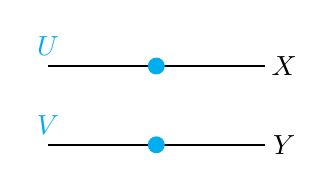
\begin{tikzpicture}[baseline = 0]
  \node (X) at (2,0.5) {$X$};
  \node (X) at (2,-0.5) {$Y$};
  \node (U) at (-1,0.75) {$\textcolor{cyan}{U}$};
  \node (V) at (-1,-0.25) {$\textcolor{cyan}{V}$};
  
  \draw[thick] (1.75,0.5) -- (-1,0.5);
  \draw[thick] (1.75,-0.5) -- (-1,-0.5);
  \draw[cyan, fill] (0.375,0.5) circle(0.1);
  \draw[cyan, fill] (0.375,-0.5) circle(0.1);
\end{tikzpicture}
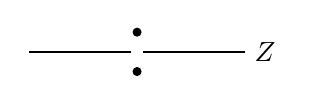
\begin{tikzpicture}[baseline = 0]
  \node (Z) at (2,0) {$Z$};
    
  \draw[thick] (1.75,0) -- (0.45,0);
  \draw[thick] (0.3,0) -- (-1,0);
  \draw[fill] (0.375,0.25) circle(0.05);
  \draw[fill] (0.375,-0.25) circle(0.05);
  
\end{tikzpicture}
\end{bsp}

%9. 5.
\begin{bspe}\begin{enumerate}[1)]\item
Quasiprojektive Variet\"aten:

$V\subseteq \IP^n(k)$, $k$ K\"orper quasi-projektiver Variet\"aten. $V$ besitzt endliceh \"Uberdeckung durch affine Variet\"aten $V= \bigcup\limits_{i=1}^r X_i$.\\
$V$ ist \quot{Verklebung} dieser affinen Variet\"aten. Jedes $X_i$ bestimmt affines Schema $\Spec k[X_i]$. Verklebe die $\Spec k[X_i]$ zu Schema $(X,\calO_X)$. $X$ hat dieselben abgeschlossenen Punkte wie $V$ (falls $k$ algebraisch abgeschlossen).

\textbf{Beobachtung:} $(X, \calO_X)$ h\"angt (bis auf Isomorphie) nicht von der gew\"ahlten affinen \"Uberdeckung ab.
\end{enumerate}\end{bspe}

\begin{Prop}
Sei $k$ algebraisch abgeschlossener K\"orper. Dann gilt:
\begin{enumerate}[a)]
\item
	Die Zuordnung $V\mapsto \Spec k[V]$ ist ein volltreuer, auf Objekten injektiver Funktor $t$ von der Kategorie der affinen Variet\"aten$/k$ in die Kategorie der affinen Schemata.
\item
	$t$ setzt sich fort zu volltreuem, auf Objekten injektivem Funktor
		\[ \text{quasiprojektive Variet\"aten}/k \to \text{ Schemata} \]
	%In der Vorlesung wurde "volltreue, auf Objekten injektiv Funktor" durch "toll" abgekuerzt, ich habe es hier ausgeschrieben.
\end{enumerate}\end{Prop}

\begin{Bez}
$\A_k^n := \Spec k[X_1,\ldots ,X_n]$ (vergleiche $\A^n(k)$)
\end{Bez}

\begin{bspe}\begin{enumerate}[1)]\item[2)]
$X=Y=\A_k^1$, $U=V=D(T) = \A_k^1 \setminus \{(T)\}$, $\A_k^1 = \Spec k[T]$. Verklebe $X$ und $Y$ l\"angs $\id: U\to V$.\\
Erhalte Schema $Z$ mit offenen Einbettungen $i_X: X\to Z$, $i_Y: Y \to Z$ sodass $Z - \{ 0_X, 0_Y\}$ isomorph zu $U=V$ ist.
\begin{center}
$i_X\left((T)\right) =: 0_X$, $i_Y\left((T)\right) =: 0_Y$
\begin{tikzpicture}
  \node (Z) at (2.25,0) {$Z$};
  \node (W) at (-0.5,1) {$\textcolor{cyan}{W}$};
  \node (KlammerRechts) at (1.5,0) {$\textcolor{cyan}{)}$};
  \node (KlammerLinks) at (-1.5,0) {$\textcolor{cyan}{(}$};
  \node (0X) at (0.5,0.6) {$0_X$};
  \node (0Y) at (0.5,-0.6) {$0_Y$};
    
  \draw[thick] (0.2,0) -- (2,0);
  \draw[thick] (-2,0) -- (-0.2,0);
  \draw[fill] (0,0.5) circle(0.05);
  \draw[fill] (0,-0.5) circle(0.05);
  
\end{tikzpicture}
\end{center}

\textbf{Es gilt:}\begin{enumerate}[(i)]
\item
	$Z$ ist irreduzibel.
\item
	Sei $W \subseteq Z$ offen, $0_X \in W$, $0_Y \in W$, $f\in \calO_Z(W)$. Dann ist $f(0_X) = f(0_Y)$.
\item
	Die Diagonale $\Delta = \{ (z_1,z_2) \in Z\times Z: z_1 = z_2\}$ ist nicht abgeschlossen.
\end{enumerate}
\textbf{Folgerung:} $Z$ ist nicht isomorph zu einem affinen Schema. Beweis in der \"Ubung.
\end{enumerate}\end{bspe}

\begin{DefBem}
Sei $S:= \bigoplus\limits_{d\ge 0} S_d$ graduierter Ring ($S_d \cdot S_e = S_{d+e}$)
\begin{enumerate}[a)]
\item
	$\Proj(S) := \{ \p \subset S: \p$ homogenes Primideal$, S_+ \nsubseteq \p\}$\\
	$(S_+:= \bigoplus\limits_{d> 0} S_d)$ hei\ss t \defterm{homogenes Spektrum}\index{Spektrum!homogenes} von $S$.
\item
	F\"ur ein homogenes Ideal $I\subseteq S$ sei $V(I): \{\p \in \Proj S, I \subseteq \p\}$. Die $V(I)$ bilden die abgeschlossenen Mengen einer Topologie auf $\Proj S$ (\defterm{Zariski Topologie}).
\item
	F\"ur homogenes $f \in S$ sei $D_+(f) := \Proj S - V(f)$. Die $D_+(f)$, $f\in S$ homogen, bilden Basis.
\item
	F\"ur $f \in S$ homogen sei
		\[ \calO_{\Proj S} (D_+(f)) := S_f^{\hom} = \left\{\frac{a}{f^d}: a \text{ homogen vom Grad } d\cdot \deg(f) \right\} \]
\item
	Es gibt genau eine Garbe $\calO_{\Proj S}$ von Ringen auf $\Proj S$ mit $\calO_{\Proj S}(D_+(f)) = S_f^{\hom}$.
\item
	F\"ur $\p \in \Proj S$ ist
		\[ \calO_{Proj S, \p} = S_\p^{\hom} = \left\{ \frac{a}{b}: a,b \text{ homogen}, \deg a = \deg b, b \notin \p \right\} \]
	\textcolor{gray}{(lokaler Ring mit maximalem Ideal $\p \cdot S_\p^{\hom} := \{ \frac{a}{b} \in S_\p^{\hom} : a \in \p \}$)}
\item
	$(\Proj S, \calO_{\Proj S})$ ist Schema.
\end{enumerate}\end{DefBem}

\begin{bew}\begin{enumerate}[a)]\item[g)]
$D_+(f), \underbrace{\calO_{\Proj S}(D_+(f))}_{\ni \p \mapsto \{ \frac{a}{f^d} \in S_f^{\hom}: a \in \p \}} \cong \Spec S_f^{\hom}$
\end{enumerate}\end{bew}

\begin{bsp}
$S= k[X_0,\ldots ,X_n]$

Dann: $\Proj S = t(\IP^n(k)) =: \IP_k^n$, denn $D_+(X_i) = \Spec k[\frac{X_0}{X_i},\ldots ,\frac{X_n}{X_i}]$
\end{bsp}
\newpage

%-------------------------- Abschnitt 4 (Abgeschlossene Unterschemata) --------------------------
%10. 5.

\section{Abgeschlossene Unterschemata}

\begin{BemDef}
Sei $R$ Ring, $I \subseteq R$ Ideal
\begin{enumerate}[a)]
\item
	Die Abbildung  $V(I) \to \Spec(\FakRaum{R}{I}), \p \mapsto \p \mod I$ ist ein Hom\"oomorphismus.
\item
	$(V(I), \calO_{\Spec (R/I)})$ hei\ss t \defterm{abgeschlossenes Unterschema}\index{Schema!abgeschlossenes Unter-} von $\Spec R$.
\item
	Die abgeschlossenen Unterschemata von $\Spec R$ entsprechen bijektiv den Idealen in $R$.
\item
	F\"ur abgeschlossene Unterschemata $Z_i \in \Spec\FakRaum{R}{I_i}$ gilt: $Z_2$ ist abgeschlossenes Unterschema von $Z_1$ (\quot{$Z_2 \le Z_1$}) $\Leftrightarrow I_1 \subseteq I_2$.\\
	Es ist dann $Z_2 = V(I_2) \subseteq V(I_1) = Z_1$
\end{enumerate}\end{BemDef}

\begin{bsp}
$X = \textcolor{red}{\A_k^1} - \Spec[X]$, $Z_1 = \Spec \FakRaum{k[X]}{(X^2)}$, $Z_2 = \textcolor{red}{\FakRaum{k[X]}{X^2-X)}}$. Dann ist $Z_1\subseteq Z_2$ als topologische R\"aume aber nicht als abgeschlossene (Unter-) Schemata.
\end{bsp}

\begin{DefBem}\label{4.2}
Sei $I \subseteq R$ Ideal, $Z = \Spec \FakRaum{R}{I}$ das zugeh\"orige abgeschlossene Unterschema von $X = \Spec R$.
\begin{enumerate}[a)]
\item
	F\"ur $U\subseteq X$ offen sei $I(U):= I \cdot \calO_X(U)$, das Bild von $I$ unter Restriktion.\\
	$\mathcal I$ ist Garbe von Idealen auf $X$.
\item
	Sei $j: Z \to X$ die Inklusion. Dann ist $j_*\calO_Z \cong \FakRaum{\calO_X}{I}$
\end{enumerate}\end{DefBem}

\begin{bew}\begin{enumerate}[a)]\item[b)]
F\"ur $f \in R$ ist $j_*\calO_ZD(f) = \calO_Z j^{-1} D(f) = \calO_Z (D(f)n\Z) = \calO_Z (D(\overline f)) = (\FakRaum{R}{I}) \overline f = \FakRaum{R_f}{IR_f} = \FakRaum{\calO_X}{I(D(f))}$
\end{enumerate}\end{bew}

\begin{Folg}
In der Situation \ref{4.2} wird $j:Z \to X$ zum Schemamorphismus, wobei 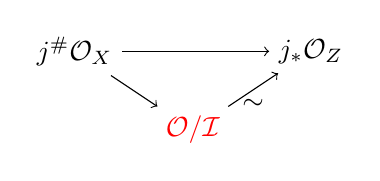
\begin{tikzpicture}[baseline=-20]\node (0) at (-1.5, 0) {$j^\#\calO_X$}; \node (1) at (1.5,0) {$j_*\calO_Z$}; \node (2) at (0, -1) {\textcolor{red}{$\calO/\mathcal I$}}; \draw[->] (0) -- (1);\draw[->] (0) -- (2);\draw[->] (2) -- node[below]{$\sim$}(1);\end{tikzpicture} die Quotientenabbildung $\calO_X \to \FakRaum{\calO_X}{\mathcal I}$ ist.
\end{Folg}

\begin{Def}
Sei $(X, \calO_X)$ ein Schema\begin{enumerate}[a)]
\item
	Eine Garbe $\calI$ (von abelschen Gruppen) auf $X$ hei\ss t \defterm{Idealgarbe}, wenn f\"ur jedes offene $U\subseteq X$ $\calI(X)$ ein Ideal in $\calO_X(U)$ ist und die Restriktionshomomorphismen $\calO_X(U)$-linear sind.
\item
	Ist $X = \Spec R$ affines Schema, so hei\ss t eine Idealgarbe $\calI$ auf $X$ \defterm{quasikoh\"arent}, wenn es ein Ideal $I$ in R gibt mit $\calI(U) = \textcolor{red}{I\calO_X(U)}$ f\"ur jedes offene $U\subseteq X$.
\item
	Eine Idealgarbe $\calI$ auf $X$ hei\ss t \defterm{koh\"arent}, wenn f\"ur jedes offene affine Unterschema $U\textcolor{red}{\subset} X$ die Einschr\"ankung $\calI|_U$ quasikoh\"arent ist.
\end{enumerate}\end{Def}

\begin{Prop}
Eine Idealgarbe $\calI$ auf $X$ ist genau dann quasikoh\"arent, wenn es eine offene \"Uberdeckung \textcolor{red}{$(U_i)_{i\in I}$} gibt durch \textcolor{red}{affine} Unterschemata \textcolor{red}{$U_i$ gibt}, sodass $\FakRaum{\calI}{U_i}$ quasikoh\"arent ist f\"ur jedes $I$. (Beweis \"Ubung)
\end{Prop}

\begin{DefBem}\begin{enumerate}[a)]
\item
	Sei $(X, \calO_X)$ ein Schema. Ein abgeschlossenes Unterschema von $X$ ist ein  Schema $(Y, \calO_Y)$, wobei $Y\subseteq X$ abgeschlossen und $\calO_Y = \textcolor{red}{\FakRaum{\calO_X}{\calI}}$ f\"ur eine quasikoh\"arente Untergarbe $\calI \subseteq \calO_X$.
\item
	Ist $(Y, \calO_Y)$ abgeschlossenes Unterschema, so gilt f\"ur jedes offene $U\subseteq X$: $U\cap Y$ ist das abgeschlossene Unterschema von $U$, das zu $\calI/U$ geh\"ort. Ist $U$ affin, so ist $\calI/U$ die von $\calI(U)$ induzierte Idealgarbe.
\end{enumerate}\end{DefBem}

\begin{DefBem}\begin{enumerate}[a)]
\item
	Sei $R$ ein Ring.\\
	$N_R := \sqrt{(0)} = \{x \in R | \exists n \ge 1: x^n = 0\}$ ist ein Ideal in $R$, das \defterm{Nilradikal}.
\item
	Ein Ring $R$ hei\ss t \defterm{reduziert}, wenn $N_R = (0)$ ist.
\item
	Ist $X = \Spec R$, so hei\ss t $X_{\Red} := \textcolor{red}{\Spec \FakRaum{R}{N_R}}$ das zu $X$ assoziierte \deftermspec{reduzierte Schema}{Schema!reduziertes}.
\item
	$X_{\Red}$ ist abgeschlossenes Unterschema von $X$ und $X_{\Red} \hookrightarrow X$ ist Hom\"omorphismus.
\item
	Sei $X$ ein Schema, $\calN_X$ die durch $\calN_X(U) =$ Nilradikal in $\calO_X(U)$ definierte Idealgarbe.\\
	Dann gilt: $\calN_X$ ist quasikoh\"arent.
\item
	Das zu $\calN_X$ assoziierte abgeschlossene Unterschema von $X$ hei\ss t $\calX_{\red}$. $(X, \calO_X)$ hei\ss t \defterm{reduziert}, wenn $\calX_{\red} \cong X$ als Schema, das hei\ss t \textcolor{red}{$\calN_X = 0$}.
\end{enumerate}\end{DefBem}

\begin{bew}\begin{enumerate}[a)]\item[e)]
\emph{Zu zeigen:} F\"ur $f \in R$, $R$ Ring, gilt: $\calN_{(R_f)} = \calN_RR_f$.\begin{twosidedproof}
\proofsupseteq
	Sei $a \in \calN_R$, also $a^n = 0$ f\"ur ein $n \ge 1$. F\"ur $x\in R_f$ ist $ax \in \calN_{R_f}$
\proofsubseteq
	$x = \frac{a}{f^{\textcolor{red}{*}}} \in R_f, x^n = 0 \Rightarrow \frac{a^n}{f^{\textcolor{red}{*}n}} = 0 \Rightarrow \textcolor{red}{a^n = 0} $
\end{twosidedproof}\end{enumerate}\end{bew}

\newpage

%-------------------------- Abschnitt 5 (Faserprodukte) --------------------------
%16. 5.

\section{Faserprodukte}

\begin{DefBem}\label{5.1}
Seien $X, Y, S$ Mengen, $f: X\to Y$, $g: Y \to S$ Abbildungen.\begin{enumerate}[a)]
\item
	$X \X_S Y := \{(x,y) \in X \X Y: f(x) = g(y)\}$ hei\ss t \defterm{Faserprodukt}.
\item
	Es gilt: $X \X_S Y = \bigcup\limits_{s \in S} f^{-1}(s) \X g^{-1}(s)$
\item\label{5.1c}
	Das Faserprodukt erf\"ullt folgende UAE:\\
	F\"ur alle Mengen $Z$, Abbildungen $\varphi: Z \to X$, $\psi: Z \to Y$ mit $f \circ \varphi = g \circ \psi$ gibt es genau eine $h: Z \to X \X_S Y$ mit $\varphi = \pr_X \circ h$, $\psi = \pr_Y \circ h$.
	\begin{center}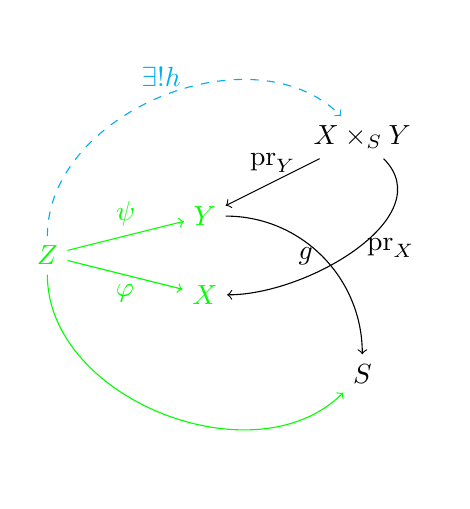
\begin{tikzpicture}
	\node (0) at (0,0) {\textcolor{green}{$Z$}};
	\node (1) at (2,0.5) {\textcolor{green}{$Y$}};
	\node (2) at (2,-0.5) {\textcolor{green}{$X$}};
	\node (3) at (4,1.5) {$X \X_S Y$};
	\node (4) at (4,-1.5) {$S$};
	
	\draw[->, green] (0) -- node[above] {$\psi$} (1);
	\draw[->, green] (0) -- node[below] {$\varphi$} (2);
	
	\draw[->, dashed, cyan] (0) to [out=90, in=135] node[above] {$\exists! h$} (3);
	\draw[->, green] (0) to [out=270, in=225] (4);
	
	\draw[->] (3) -- node[above] {$\pr_Y$} (1);
	\draw[->] (3) to [out=315, in=0] node[right] {$\pr_X$} (2);
	\draw[->] (1) to [out=0, in=90] node[left] {$g$} (4);
	\end{tikzpicture}\end{center}
\item
	Das Faserprodukt ist der Limes des Diagramms
	\begin{center}\begin{tikzpicture}
	\node (0) at (-1.5,0) {$X$};
	\node (1) at (1.5,0) {$Y$};
	\node (2) at (0,-1) {$S$};
	
	\draw[->] (0) -- node[below] {$f$} (2);
	\draw[->] (1) -- node[below] {$g$} (2);
	\end{tikzpicture}\end{center}
\end{enumerate}\end{DefBem}

\begin{bew}\begin{enumerate}[a)]\item[c)]
Setze $h(z):= (\varphi(z), \psi(z))$
\end{enumerate}\end{bew}

\begin{bspe}\begin{enumerate}[1)]
\item
	$S= \{s\} \Rightarrow X \X_S Y = X \X Y$
\item
	$X\subseteq S, Y \subseteq S$, $f,g$ die Inklusionen $\Rightarrow X \X_S Y = X \cap Y$
\item
	$Y \subseteq S$, $g: Y \hookrightarrow S \Rightarrow X \X_S Y = f^{-1}(Y)$
\item
	$X=Y \Rightarrow X \X_S Y =$ Equalizer$(f,g)$
\end{enumerate}\end{bspe}

\begin{Def}
Seien $X, Y, S$ Schemata, $f: X \to S, g: Y \to S$ Morphismen.\\
Dann hei\ss t ein Schema $X \X_S Y$ zusammen mit Morphismen $\pr_X: X \X_S Y \to X$ und $\pr_Y: X \X_S Y \to Y$, sodass $f \circ \pr_X = g\circ \pr_Y$ ist, \defterm{Faserprodukt} von $X$ und $Y$ \"uber $S$, wenn die UAE aus \ref{5.1} \ref{5.1c}) erf\"ullt ist.
\end{Def}

\begin{DefBem}
Sei $S$ ein Schema.\begin{enumerate}[a)]
\item
	Ein \defterm{S-Schema} ist ein Schema $X$ zusammen mit einem Morphismus $f:X \to S$.
\item
	Die $S$-Schmata bilden eine Kategorie \underline{Sch/$S$}.
\item
	Das Faserprodukt $X \X_S Y$ ist das Produkt von $f: X \to S$ und $g: Y \to S$ in \underline{Sch/$S$}.
\end{enumerate}\end{DefBem}

\begin{bsp}
$S = \Spec$, $k$ K\"orper

Ein Morphismus $X \to \Spec k$ ist nach \"Ubung 3, Aufgabe 1 vollst\"andig bestimmt durch einen Ringhomomorphismus $k \to \calO_X(X)$. Dieser macht $\calO_X(X)$ zur $k$-Algebra und $\calO_X$ zu einer Garbe von $k$-Algebren. Insbesondere sind $k$-Variet\"aten \"uber den Funktor $t$ $k$-Schemata. Das Faserprodukt von $k$-Variet\"aten ist das Produkt der $k$-Variet\"aten (im Sinne von Algebraische Geometrie I)(siehe unten).
\end{bsp}

\begin{Satz}
Das Faserprodukt $X \X_S Y$ existiert f\"ur alle $S$-Schemata $f: X \to S$ und $g: Y \to S$. Es ist eindeutig bis auf eindeutigen Isomorphismus.
\end{Satz}

\begin{bew}\begin{enumerate}[(1)]
\item
	$X= \Spec A$, $Y =\Spec B$, $S =\Spec R$ affin. $f$ und $g$ machen $A$ und $B$ zu $R$-Algebren.
	
	\emph{Behauptung:} Das Tensorprodukt $A \otimes_R B$ erf\"ullt $\Spec (A \otimes_R B) = X \X_S Y$.
	
	\emph{Erinnerung:} Das Tensorprodukt $M \otimes_R N$ von $R$-Moduln $M,n$ \quot{linearisiert} die bilinieare Abbildung
	\begin{center}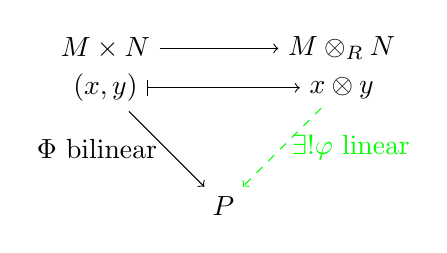
\begin{tikzpicture}
	\node (0) at (-1.5,0) {$M\X N$};
	\node (1) at (1.5,0) {$M\otimes_R N$};
	
	\node (2) at (-1.5,-0.5) {$(x,y)$};
	\node (3) at (1.5,-0.5) {$x\otimes y$};
	
	\node (4) at (0, -2) {$P$};
	
	\draw[->] (0) -- (1);
	\draw[|->] (2) -- (3);
	
	\draw[->] (2) -- node[left] {$\Phi$ bilinear}(4);
	\draw[->, dashed, green] (3) -- node[right] {$\exists! \varphi$ linear} (4);
	\end{tikzpicture}\end{center}
	
	\begin{enumerate}[\textbullet]
	\item
		Sind $M=A$ und $N=B$ $R$-Algebren, so hat $A \otimes_R B$ eine Struktur als $R$-Algebra:
			\[(a_1 \otimes b_1) \cdot (a_2 \otimes b_2) := a_1a_2 \otimes b_1b_2\]
	\item
		$\begin{array}{l} \sigma_A: A \to A \otimes_R B, a \mapsto a \otimes 1 \\ \sigma_B: B \to A \otimes_R B, b \mapsto 1 \otimes b \end{array}$ sind $R$-Algebren-Homomophismen.
	\item
		$A \otimes_R B$ erf\"ullt die richtige UAE
		\begin{center}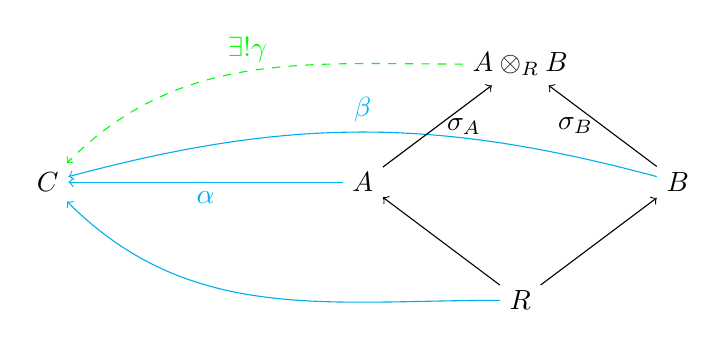
\begin{tikzpicture}
		\node (0) at (-4, 0) {$C$};
		\node (1) at (0, 0) {$A$};
		\node (2) at (4, 0) {$B$};
		
		\node (3) at (2, 1.5) {$A \otimes_R B$};
		\node (4) at (2, -1.5) {$R$};
		
		\draw[->, cyan] (1) -- node[below] {$\alpha$} (0);
		\draw[->, cyan] (2) to [in=15, out=165] node[above] {$\beta$} (0);
		
		\draw[->] (4) -- (1);
		\draw[->] (4) -- (2);
		\draw[->] (1) -- node[right] {$\sigma_A$} (3);
		\draw[->] (2) -- node[left] {$\sigma_B$}(3);
		
		\draw[->, cyan] (4) to [in=315, out=180] (0);
		\draw[->, dashed, green] (3) to [in=45, out=180] node[above] {$\exists! \gamma$} (0);
		\end{tikzpicture}\end{center}
		\quot{Beweis:} $\tilde \gamma: A \X B \to C$, $(a,b) \mapsto \alpha(a) \cdot \beta(b)$ ist bilinear, induziert also $\gamma: A \otimes B \to C$ linear. Nachrechnen: $\gamma$ Ringhomomorphismus, $\gamma$ eindeutig.
	\end{enumerate}
	\emph{Also:} $\Spec(A \otimes_R B)$ erf\"ullt die geforderte UAE f\"ur alle affinen Schemata $Z$.
	
	Ist $Z$ beliebiges Schema, so induzieren $\varphi: Z \to X$ und $\psi: Z \to Y$ $R$-Algebrahomomorphismen $\alpha: A \to \calO_Z(Z)$, $\beta: B \to \calO_Z(Z)$.\\
	$\alpha$ und $\beta$ induzieren $\gamma: A\otimes_R B \to \calO_Z(Z)$, also (\"Ubung 3, Aufgabe 1) Morphismus $h: Z \to \Spec (A \otimes_R B)$.
\item
	$X,Y,Z$ nicht notwendig affin.\\
	\"Uberdecke $S$ durch offene affine Schemata $S_i = \Spec R_i$ ($i\in I$). Sei $X_i:= f^{-1}(S_i)$, $Y_i:= g^{-1}(S_i)$ (offen in $X$ bewziehungsweise $Y$).\\
	\"Uberdecke $X_i$ durch offene affine Schemata $X_{ij} = \Spec A_{ij}$\\
	\"Uberdecke $Y_i$ durch offene affine Schemata $Y_{ij} = \Spec B_{ij}$\\
	Nach (1) existiert $X_{ij} \otimes_{S_i} Y_{ik}$ f\"ur alle $i,j,k$
	
	\emph{Behauptung 1:} Sei $T$ ein Schema, $V,W$ $T$-Schemata, $(V_l)_{l\in L}$ offene \"Uberdeckung von $V$. Existiert $V_l \X_T W$ f\"ur jedes $l$, so existiert $V \X_T W$.
	
	Wende Behauptung 1 an auf\begin{itemize}
	\item
		$T=S_i$, $V = X_i$, $W=Y_{ik}$, $V_l=X_{il}$ $\Rightarrow X_i \X_{S_i} Y_{ik}$ existiert $\forall i,k$
	\item
		$T=S_i$, $V = Y_i$, $W=X_{i}$, $V_l=Y_{il}$ $\Rightarrow X \X_{S_i} Y_{ik}$ existiert $\forall i$
	\end{itemize}

	\emph{Behauptung 2:} F\"ur jedes $i$ ist $X_i \X_{S_i} Y_i = X_i \X_{S} Y$
	
	Dann wende Behauptung an auf
		\[ T=S, V=X, W=Y, V_l = X_l \Rightarrow X \X_S Y \text{ existiert} \]
	
	\emph{Beweis 2:}
	\begin{center}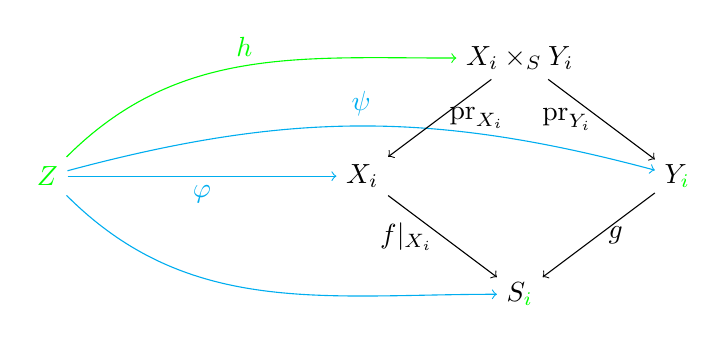
\begin{tikzpicture}
		\node (0) at (-4, 0) {\textcolor{green}{$Z$}};
		\node (1) at (0, 0) {$X_i$};
		\node (2) at (4, 0) {$Y_{\textcolor{green}{i}}$};
		
		\node (3) at (2, 1.5) {$X_i \X_S Y_i$};
		\node (4) at (2, -1.5) {$S_{\textcolor{green}{i}}$};
		
		\draw[->, cyan] (0) -- node[below] {$\varphi$} (1);
		\draw[->, cyan] (0) to [in=165, out=15] node[above] {$\psi$} (2);
		
		\draw[->] (1) -- node[left] {$f|_{X_i}$} (4);
		\draw[->] (2) -- node[right] {$g$}(4);
		\draw[->] (3) -- node[right] {$\pr_{X_i}$} (1);
		\draw[->] (3) -- node[left] {$\pr_{Y_i}$}(2);
		
		\draw[->, cyan] (0) to [in=180, out=315] (4);
		\draw[->, green] (0) to [in=180, out=45] node[above] {$h$} (3);
	\end{tikzpicture}\end{center}
		\[ \Psi(Z) \subseteq g^{-1} (\underbrace{f (\overbrace{\varphi(Z)}^{\subseteq X_i} )}_{\subseteq S_i} ) \subseteq Y_i \]
	\emph{Beweis 1:} Verklebe die $V_l \X_T W$ l\"angs $U_{lm} = \pr_l^{-1} (V_l \cap V_m) \subseteq V_l \X_T W$. Es gilt: $U_{lm} = (V_l \cap V_m) \X_T W$. Dann ist $U_{lm} \quot{=} U_{ml}$, lassen sich also verkleben zu Schema $V$. Zeige: $\tilde V = V \X_T W$
\end{enumerate}\end{bew}


%-_-_-_-_-_-_-_-_-_-_-_-_-_-_ Anhang -_-_-_-_-_-_-_-_-_-_-_-_-_-_-_-_


\appendix

\def\indexspace{\par\medskip}
%\printindex[default]
\printindex[default][\phantomsection\addcontentsline{toc}{chapter}{Stichwortverzeichnis}\vspace{-1.2em}]


%-_-_-_-_-_-_-_-_-_-_-_-_-_-_ Uebungen -_-_-_-_-_-_-_-_-_-_-_-_-_-_-_-_

\chapter{\"Ubungen}

% Die Benennung der "section" so aendern, dass "\"Ubung 123 vom " am Anfang steht
% Der Code ist fast genau der vom Anfang der Praeambel, dort steht die Erklaerung
\renewcommand*{\othersectionlevelsformat}[3]{\ifstr{#1}{section}{\"Ubung\ #3\ vom\ }{#3\autodot\enskip}}

% Das Format der "section" in Kopfzeile der rechten Seiten
\renewcommand*{\sectionmarkformat}{\"Ubung \thesection\autodot\ vom\enskip}

\setcounter{section}{-1}

%-------------------------- Uebung 0 --------------------------
\section{24. April 2012}
\setcounter{Aufg}{0} %Damit die Aufgaben jedes Mal bei Aufgabe 1 anfangen
\setcounter{Loes}{0}

\begin{Aufg}
 Sei $X$ ein topologischer Raum, $A$ eine abelsche Gruppe und $x \in X$. 

Die "`Wolkenkratzergarbe"' auf $X$ ist definiert durch 
$\mathcal{W}(U) \coloneqq \left\{ \begin{array}{ll}
                                   A & ,\, x \in U\\
                                   \{0\} & ,\,x \notin U
                                  \end{array}
\right.$ f\"ur $U \subseteq X$ offen, mit Restriktionsabbildungen 
$$\rho_V^U = \left\{ \begin{array}{rcll}
                     \{0\} \ni &0 \mapsto 0& \in \{0\}& ,\, x \notin V,\, x \notin U\\
                     A \ni &a \mapsto 0& \in \{0\}& ,\, x \notin V,\, x \in U\\
                     & \id_A && ,\,x \in V,\, x \in U
                    \end{array} \right.$$ f\"ur $V \subseteq U \subseteq X$ offen.
\begin{enumerate}%[topsep=0cm, parsep=0cm, label=\alph*)]
 \item Zeige, dass $\mathcal{W}$ eine Garbe von abelschen Gruppen auf $X$ ist.
 \item Berechne die Halme der Garbe.
\end{enumerate}
\end{Aufg}



\begin{Aufg}
 Sei $X$ ein topologischer Raum und $\mathcal{F}$ eine Pr\"agarbe von abelschen Gruppen auf $X$. Ist $x \in X$ ein Punkt, so bezeichne $\mathcal{F}_x$ den Halm von $\mathcal{F}$ in $x$. Nun definiert man die Menge
\begin{center}
Sp\'e$(\mathcal{F}):= \stackrel{.}{\bigcup\limits_{x\in X}} \mathcal{F}_x$.
\end{center}
Definiere weiter eine Projektionsabbildung
$\pi \colon \textup{Sp\'e}(\mathcal{F}) \rightarrow X$ durch $\mathcal{F}_x \ni s \mapsto x$. \\
F\"ur jede offene Menge $U \subseteq X$ und f\"ur jedes $s \in \mathcal{F}(U)$ erh\"alt man eine Abbildung $\overline{s} \colon U \rightarrow \textup{Sp\'e}(\mathcal{F})$ durch
$x \mapsto s_x$, wobei $s_x$ der Keim von $s$ in $x$ sei. Alle diese Abbildungen sind Schnitte von $\pi$ \"uber $U$, d.\,h. f\"ur jedes dieser $\overline{s}$ gilt: $\pi \circ \overline{s} = \textup{id}_U$.
Nun macht man Sp\'e$(\mathcal{F})$ zu einem topologischen Raum, indem man ihm die feinste Topologie gibt, so dass alle diese $\overline{s}$ f\"ur alle $s$ und alle $U$ stetig werden. Versehen mit dieser Topologie hei\ss t $\textup{Sp\'e}(\mathcal{F})$ der \textit{Espace Etal\'e} zur Pr\"agarbe $\mathcal{F}$.

Sei nun $\mathcal{F}^+$ die zu $\mathcal{F}$ assoziierte Garbe. Zeige:\\
F\"ur jede offene Menge $U \subseteq X$ ist $\mathcal{F}^+(U)$ die Menge aller \textbf{stetigen} Schnitte von $\pi$ \"uber $U$.
 Insbesondere ist $\mathcal{F}$ genau dann eine Garbe, wenn f\"ur jedes offene $U \subseteq X$ die Menge aller stetigen Schnitte von $\pi$ \"uber $U$ gerade $\mathcal{F}(U)$ ist.
\end{Aufg}




\begin{Loes}\begin{enumerate}[a)]
\item
  Sei $U$ offen, $U = \bigcup\limits_{i\in I} U_i$, $s_i$ konsistente Familie.
  \begin{description}[\setlabelstyle{\itshape}]
  \item[Fall 1:]
    $x \in U \Rightarrow \exists i \in I: x\in U_i \Rightarrow \calW(U_i) = A \Rightarrow  \calW(U) = A$\\
    \emph{Behauptung:} $s=s_i$ ist Amalgam\\
    $\rho_{U_i}^U= \id_A \leadsto s = s_i$ ist einziger Kandidat\\
    F\"ur $j\in I$\begin{description}
    \item{$\bullet$ mit $x\in U_j$:}\\
      $s_j = \id_A(s_j) = \rho_{U_i\cap U_j}^{U_j}(s_j) = \rho_{U_i\cap U_i}^{U_j}(s_j)$\\
      $\textcolor{white}{s_j = \id_A(s_j)}= \id_A(s_i) = s_i = s = \rho_{U_j}^U(s)$
    \item{$\bullet$ mit $x\notin U_j$:}\\
      $s_j = 0, \rho_{U_0}^U(s) = 0$
    \end{description}
  \item[Fall 2:]
    $x \notin U \Rightarrow x\notin U_j \forall j \in I$\\
    $\Rightarrow \calW(U) = \calW(U_j) = \{0\}$
  \end{description}
\item
  Sei $y \in X$. Bestimme den Halm von $\calW$ in $y$.\\
  $\calW_y = \{[(U,s)]_y \vert s\in \calW(U)\}$ mit $[(U,s)]_y = [(U',s')]_y \Leftrightarrow \exists U'' \subseteq U \cap U', y \in U'': s|_{U''} = s'|_{U''}$ \begin{description}[\setlabelstyle{\itshape}]
  \item[Fall 1:]$\exists U\subseteq X$ offen, $y\in U, x\notin U$\\
    $\Rightarrow [U',s] = [U,0]$ f\"ur alle $U'\subseteq X$ offen, $s\in \calW(U')$\\
    $\Rightarrow \calW_y = \{0\}$
  \item[Fall 2:] $\forall$ offenen Umgebungen $U$ von $y: x\in U$\\
    $\Rightarrow \calW_y \cong A$, \emph{denn:} Sei $U$ offene Umgebung von $y$
      \begin{equation*}\begin{split} \varphi:&\left\{\begin{array}{rcl} A &\to& \calW_y \\
      a &\mapsto& [U,a]\end{array}\right.\\
      \psi:& \left\{\begin{array}{rcl} \calW_y &\to& A \\
      \,[U,a] &\mapsto& a\end{array}\right.\end{split}\end{equation*}
    $[U,a]_y = [U,b]_y \Leftrightarrow a=a|_{U''} = b|_{U''} = b$
  \end{description}
  
\end{enumerate}\end{Loes}

\begin{Loes}
\begin{minipage}[t]{0.6\textwidth}
$s\in \calF(U), x\in U \leadsto [U,s]_x \in \calF_x$\\
$\bar s :\left\{\begin{array}{rcl}U &\to& \Spe(\calF)\\ x &\mapsto& [U,s]_x\in\calF_x\end{array}\right., \pi \circ \bar s = \id_U$\end{minipage}
\begin{minipage}[c]{0.4\textwidth}
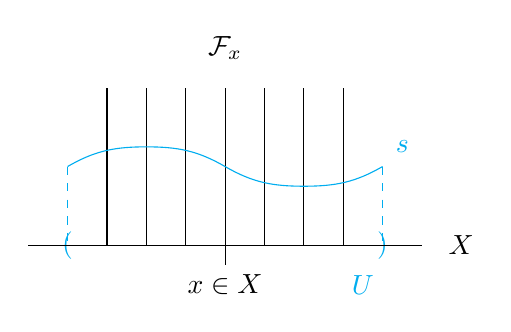
\begin{tikzpicture}
  %Punkte definieren
  \node (x) at (0,-0.5){$x \in X$};
  \node (Fx) at (0,2.5){$\calF_x$};
  \node (s) at (2.25,1.25){\textcolor{cyan}{$s$}};
  \node (X) at (3,0){$X$};
  \node (KlAuf) at(-2,0) {\textcolor{cyan}{(}};
  \node (KlZu) at(2,0) {\textcolor{cyan}{)}};
  \node (U) at(1.75,-0.5) {\textcolor{cyan}{$U$}};

  \draw (-2.5,0) -- (2.5,0);
  %senkrechte Linien zeichnen
  \draw (-1.5,0) -- (-1.5,2);
  \draw (-1,0) -- (-1,2);
  \draw (-0.5,0) -- (-0.5,2);
  \draw (0,-0.25) -- (0,2);
  \draw (1.5,0) -- (1.5,2);
  \draw (1,0) -- (1,2);
  \draw (0.5,0) -- (0.5,2);
  %Schlangenlinie
  \draw[cyan] (-2,1) to [out=30,in=180] (-1,1.25) to [out=0,in=150] (0,1) to [out=330,in=180] (1,0.75) to [out=0,in=210] (2,1);
  %gestrichelte Linien
  \draw[dashed,cyan] (-2,1) -- (-2,0);
  \draw[dashed,cyan] (2,1) -- (2,0);
\end{tikzpicture}
\end{minipage}
$\calF^+$ assoziiert Garbe zu $\calF$, also f\"ur $U\subseteq X$ offen:
  \[\begin{array}{rccr}\calF^+(U) &:= \{s: U\to \dot{\bigcup\limits_{x\in U}}\calF_x &\vert& \forall x\in X: s(x)\in \calF_x \text{ und } \exists \text{ offene Umgebung } U_x \\ &&& \text{ von } x, \exists f\in \calF(U_x), s(y) = f_y := [(U_x,f)]_y\}\end{array}\]
\emph{Zu zeigen:} $\calF^+(U) = \{\text{stetige Schnitte von } \pi \text{ \"uber } U\}$
\begin{twosidedproof}
\proofsubseteq
  Sei $s\in \calF^+(U)$\\
  $\pi \circ s = \id \Rightarrow s$ Schnitt\\
  Noch zu zeigen: $s$ ist stetig\\
  Nach Definition von $\calF^+$ gibt es \"Uberdeckung $U = \bigcup\limits_{i \in I} U_i$ und Schnitte $s_i \in\calF(U_i)$ mit $s|_{U_i} = \bar{s_i}$. Die $\bar{s_i}: U_i \to \Spe(\calF)$ sind stetig.\\
  Sei $\widetilde U \subseteq \Spe(\calF)$ offen.\\
  $\bar s_i^{-1}(\widetilde U) = s^{-1}(\widetilde U) \cap U_i$ offen\\
  $s^{-1}(\widetilde U) = \bigcup\limits_{i\in I} (s^{-1}(\widetilde U)\cap U_i)$ ist offen
\proofsupseteq
  Sei $s: U\to \Spe(\calF)$ stetiger Schnitt von $\pi$ \"uber $U$, das hei\ss t $\forall x \in X: s(x) \in \calF_x$.\\
  \emph{Noch zu zeigen:} $\forall x\in X \exists U_x\in \Off(X)$ mit $x\in U_x$ und ein $f\in \calF(U_x)$ sodass $\forall y \in U$ gilt $s(y) = f_y$\\
  Sei $x\in X$, $s(x)=[U',s']_x\in\calF_x$, $s'\in\calF(U')$\\
  $\widetilde U:= \{[U',s']_y \in \calF_y | y\in U'\}$ ist offen in $\Spe(\calF)$ und enth\"alt $s(x)$.
    \[[U',s']_y = [U'',s'']_y\]
  $\Rightarrow \exists U''' \subseteq U'\cap U'': s'|_{U'''} = s''|_{U'''}$\\
  $s''^{-1}(\widetilde U \cap s'(U''')) = s'^{-1}(\widetilde U \cap s'(U'''))$ offen\\
  Setze $U_x:= s^{-1}(\widetilde U)$\\
  $s$ stetig $\Rightarrow U_x$ offen, $x\in U_x$\\
  Au\ss erdem: $\forall y \in U_x: \bar{s'}(y) = \underbrace{[U', s']_y}_{=[U_x, s'|_{U_x}]_y} \xlongequal{\pi \circ s = \id} s(y)$\\
  $\Rightarrow s'|_{U_x} \in \calF(U_x)$ erf\"ullt Garbeneigenschaft.
\end{twosidedproof}

\textbf{zur L\"osung:}

In der \"Ubung wollte ich zeigen, dass f\"ur offenes $U' \subseteq X$ mit $x \in U'$ und $s' \in \mathcal{F}(U')$ die Menge $\tilde{U} \coloneqq \{ [U',s']_y \in \mathcal{F}_y \mid y \in U' \}$ offen ist bez\"uglich der oben definierten Topologie auf Sp\'e$(\mathcal{F})$.

Auf einmal scheint das Argument auf meinem Zettel wieder zu stimmen (war nur etwas knapp formuliert), deshalb schreibe ich es hier nochmal ausf\"uhrlicher auf.

Zu zeigen ist ja, dass f\"ur jedes offene $U'' \subseteq X$ und jedes $s'' \in \mathcal{F}(U'')$ die Menge $\left(\overline{s''}\right)^{-1}\left(\tilde{U}\right)$ offen in $X$ ist. Sei also $U'' \in \Off(X)$ und $s'' \in \mathcal{F}(U'')$.

Ist $\left(\overline{s''}\right)^{-1}\left(\tilde{U}\right) = \emptyset$, so ist nichts weiter zu zeigen, da $\emptyset$ ja offen ist. Ist andernfalls $y \in \left(\overline{s''}\right)^{-1}\left(\tilde{U}\right)$, so ist $ \overline{s''}(y) \in \tilde{U}$ und wegen $\overline{s''}(y) \in \mathcal{F}_y$ folgt $[U'',s'']_y = [U',s']_y$ ($\tilde{U}$ enth\"alt ja pro Halm h\"ochstens ein Element). Folglich existiert ein offenes $U''' \subseteq U' \cap U''$ mit $y \in U'''$ und $s'|_{U'''} = s''|_{U'''}$. Somit ist $U''' \subseteq \left(\overline{s''}\right)^{-1}\left(\tilde{U}\right)$ eine offene Umgebung von $y$ und $\left(\overline{s''}\right)^{-1}\left(\tilde{U}\right)$ offen.

\end{Loes}

%-------------------------- Uebung 1 --------------------------
\newpage
\section{1. Mai 2012}
\setcounter{Aufg}{0}
\setcounter{Loes}{0}

\begin{Aufg}[4 Punkte]
\begin{enumerate}[a)]
 \item Sei $X:=\{0,1\}$ mit der diskreten Topologie versehen (d.\,h. jede Teilmenge ist offen).
Bestimme alle Garben $\mathcal{F}$ von Mengen auf $X$.
 \item Bestimme die Halme $\mathcal{F}_x$ der Garben $\mathcal{F}$ aus Teil a) in den Punkten $x=0$ und $x=1$.
\end{enumerate}
\end{Aufg}

\begin{Aufg}[4 Punkte]
Sei $X$ ein topologischer Raum und $\mathcal{F}$ die Pr\"agarbe der konstanten Funktionen auf $X$. Genauer sei f\"ur $U \subseteq X$ offen 
$\mathcal{F}(U) \coloneqq \{ \, f \colon U \to \Z \mid f \textrm{ ist konstant } \}$ und f\"ur $V \subseteq U \subseteq X$ offen $\rho_V^U\colon \mathcal{F}(U) \to \mathcal{F}(V), f \mapsto f|_{V}$.
\begin{enumerate}[a)]%[topsep=0cm, parsep=0cm, label=\alph*)]
\item Zeige, dass $\mathcal{F}$ im allgemeinen keine Garbe ist.
\item Berechne die zu $\mathcal{F}$ assoziierte Garbe $\mathcal{F}^+$.
\end{enumerate}
\end{Aufg}

\begin{Aufg}[4 Punkte]
Sei $X$ ein topologischer Raum und $\mathcal{B}$ eine Basis\footnote{d.\,h. alle offenen $U \subseteq X$ lassen sich als Vereinigung von Elementen aus $\mathcal{B}$ schreiben} der Topologie von $X$. Weiter sei $\mathcal{C}$ eine Kategorie.
Wir definieren eine $\mathcal{B}$-Garbe auf $X$ als kontravarianten Funktor $\mathcal{F}'$ von $(\mathcal{B}, \subseteq)$ nach $\mathcal{C}$, der die $\mathcal{B}$-Garbeneigenschaft erf\"ullt:

Sind $U = \bigcup_{i\in I} U_i$ mit $U, U_i \in \mathcal{B}$ und $(s_i)_{i \in I}$ mit $s_i \in \mathcal{F}'(U_i)$ gegeben, so dass $\rho^{U_i}_V(s_i) = \rho^{U_j}_V(s_j)$ f\"ur alle $V \subseteq U_i \cap U_j, V \in \mathcal{B}$ gilt, dann existiert genau ein $s \in \mathcal{F}'(U)$ mit $\rho^{U}_{U_i}(s) = s_i$ f\"ur alle $i \in I$.

Sei zun\"achst $\mathcal{C}$ die Kategorie der Mengen. 
\begin{enumerate}[a)]%[topsep=0cm, parsep=0cm, label=\alph*)]
 \item Zeige, dass sich $\mathcal{F}'$ eindeutig zu einer Garbe $\mathcal{F}$ auf $X$ fortsetzen l\"asst.\\
  \textit{Hinweis:} Inverser Limes
 \item Es seien $\mathcal{F}$ und $\mathcal{G}$ Garben auf $X$ und f\"ur $U \in \mathcal{B}$ Abbildungen $\tilde{\varphi}(U)\colon \mathcal{F}(U) \to \mathcal{G}(U)$ gegeben, die mit den Restriktionsabbildungen $\rho^U_{U'}$ kommutieren. 
 
 Zeige, dass es einen eindeutigen Garbenmorphismus $\varphi\colon \mathcal{F} \to \mathcal{G}$ gibt mit $\varphi(U) = \tilde{\varphi}(U)$ f\"ur alle $U \in \mathcal{B}$.
 \item Mache dir klar, dass a) und b) auch in der Kategorie der (abelschen) Gruppen, der Ringe und der $R$-Moduln gelten.
\end{enumerate}
\end{Aufg}

\begin{Loes}
\begin{enumerate}[a)]%[topsep=0cm, parsep=2mm, label=\alph*)]
 \item Die offenen Mengen von $X$ sind $\Off(X)= \{ \emptyset, \{0\}, \{1\}, \{0,1\}\}$. Eine Garbe von Mengen auf $X$ ordnet jedem Element aus $\Off(X)$ eine Menge zu, also 
$$
\emptyset  \rightarrow  M_\emptyset,  \quad
\{0\}  \rightarrow  M_0,\quad
\{1\} \rightarrow  M_1,\quad
X  \rightarrow  M_X.
$$
Zus\"atzlich brauchen wir noch Restriktionsabbildungen
$$
M_0 \rightarrow  M_\emptyset,\quad
M_1  \rightarrow  M_\emptyset,\quad
M_X  \rightarrow  M_\emptyset,\quad
M_X  \rightarrow  M_0,\quad
M_X  \rightarrow  M_1,\quad
$$
so dass das folgende Diagramm kommutiert:
\begin{center}
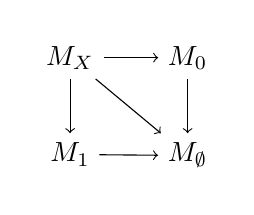
\begin{tikzpicture}
   \matrix (m) [matrix of math nodes, row sep=2em, column sep=2em]
  { M_X & M_0 \\ M_1 & M_\emptyset \\};
  \path[->]
  (m-1-1) edge (m-2-1)
      edge (m-1-2)
      edge (m-2-2)
  (m-2-1) edge (m-2-2)
  (m-1-2) edge (m-2-2);
\end{tikzpicture}
\end{center}
In der Vorlesung wurde bewiesen, dass $M_\emptyset$ einelementig sein muss. Dann kommutiert das obige Diagramm automatisch.

Da die offenen Mengen $\{0\}$ und $\{1\}$ die offene Menge $\{0,1\}$ \"uberdecken, besagt die Garbeneigenschaft, dass es zu jedem $a \in M_0$ und jedem $b\in M_1$ ein eindeutig bestimmtes $c \in M_X$ geben muss mit $\rho^X_{\{0\}}(c) = a$ und $\rho^X_{\{1\}}(c)=b$. Das bedeutet, dass $M_X \cong M_0 \times M_1$ ist. Damit haben wir alle Garben von Mengen auf $X$ charakterisiert.

 \item Der Halm der Garbe $\mathcal{F}$ in $x$ ist definiert als 
\begin{eqnarray*}
\mathcal{F}_x \coloneqq \{\, (U,f) \mid U \in \Off(X), x \in U, s \in \mathcal{F}(U) \,\}/\sim,
\end{eqnarray*}
wobei zwei Paare $(U,s)$ und $(U',s')$ \"aquivalent sein sollen, wenn es ein $U'' \subseteq U \cap U'$ gibt mit $\rho^U_{U''}(s) = \rho^{U'}_{U''}(s')$.

Zwei Punkte $(X,(a,b))$ und $(X,(a',b'))$ beschreiben genau dann den gleichen Punkt in $\mathcal{F}_0$, wenn $a = \rho^X_{\{0\}}((a,b)) = \rho^{X}_{\{0\}}((a',b'))=a'$.
Also ist $\mathcal{F}_0 \cong M_0$. Ebenso ist $\mathcal{F}_1 \cong M_1$.
\end{enumerate}
\end{Loes}

\begin{Loes}
\begin{enumerate}[a)]%[topsep=0cm, parsep=2mm, label=\alph*)]
 \item Falls es in $X$ offene Mengen $U$ und $U'$ gibt mit $U \cap U' = \emptyset$, dann ist $\mathcal{F}$ keine Garbe:
 
 Seien $f_1 \in \mathcal{F}(U)$ mit $f_1 \equiv 1$ und $f_2 \in \mathcal{F}(U')$ mit $f_2 \equiv 2$. Da $U \cap U' = \emptyset$, ist $f_1|_{U \cap U'} = {f_2}|_{ U \cap U'}$ und $(f_i)_{i\in \{1,2\}}$ ist eine konsistente Familie f\"ur die offene \"Uberdeckung $U \cup U'$. Da aber f\"ur $f \in \mathcal{F}(U \cup U')$ nicht gleichzeitig $f|_U \equiv 1$ und $f|_{U'} \equiv 2$ gelten kann, gibt es zu der konsistenten Familie kein Amalgam.
 
 \item Zun\"achst berechnen wir die Halme von $\mathcal{F}$: 
 $$[(U,f)]_x = [(U',f')]_x \Leftrightarrow \exists U'' \subseteq U \cap U' \textrm{ mit } x \in U'' : f|_{U''} = f'|_{U''} \Leftrightarrow f(x) = f'(x)$$
 Die Halme sind also \"uber $[(U,f)]_x \mapsto f(x)$ alle isomorph zu $\Z$.
 
 Es gilt 
 $$\begin{array}{cl}
    \mathcal{F}^+(U) \coloneqq \{ \, s \colon U \to \stackrel{.}{\bigcup\limits_{x \in U}} \mathcal{F}_x \mid 
    & \forall x \in U : s(x) \in \mathcal{F}_x \textrm{ und } \exists \textrm{ offene Umgebung } U_x \textrm{ von } x, \\
    & \exists f \in \mathcal{F}(U_x) \, \forall y \in U_x : s(y) = [(U_x,f)]_y \eqqcolon f_y \, \} \, .
   \end{array}$$
 Benutzen wir die Isomorphismen $\mathcal{F}_x \ni [(U,f)]_x \mapsto f(x) \in \Z$ der Halme mit $\Z$, sowie die Tatsache, dass $f \in \mathcal{F}(U_x)$ konstant ist, so besagt die letzte Bedingung an $s$:
 $$\forall x \in U \; \exists \textrm{ offene Umgebung } U_x \textrm{ von } x: \forall y \in U_x: s(y) = s(x) \, .$$
 Damit gilt
  $$\begin{array}{rcccl}
    \mathcal{F}^+(U) &= \{ & s \colon U \to \Z &\mid 
    & \forall x \in U \, \exists U_x \in \Off(X), x \in U_x : s|_{U_x} \textrm{ ist konstant}\, \}\\
    &= \{ & s \colon U \to \Z & \mid & s \textrm{ ist lokal konstant} \, \} \, .
   \end{array}$$
\end{enumerate}
\end{Loes}

\begin{Loes}
\begin{enumerate}[a)]%[topsep=0cm, parsep=0.1cm, label=\alph*)]
 \item Wir nutzen den Hinweis und definieren $\F$ mit Hilfe des inversen Limes. F\"ur $U \in \Off(X)$ setzen wir 
 $$\begin{array}{rcl}
    \F(U) &\coloneqq& \varprojlim\limits_{V \subseteq U, V \in \mathcal{B}} \F'(V) \\
    &=& \{ \, (s_V)_{V \subseteq U, \, V \in \mathcal{B}} \in \prod_{V \subseteq U, V \in \mathcal{B}} \F'(V) \mid \forall W \subseteq V \subseteq U, V,W \in \mathcal{B}: \rho^V_W(s_V) = s_W \, \}
   \end{array}
$$
und f\"ur $U' \subseteq U \subseteq X$ offen sei
$$
\rho^U_{U'} \colon \F(U) \to \F(U'), (s_V)_{V \subseteq U, V \in \mathcal{B}} \mapsto (s_V)_{V \subseteq U', V \in \mathcal{B}}\,.
$$
Die Abbildung $\rho^U_{U'}$ bildet die Familie $(s_V)_{V \subseteq U, V \in \mathcal{B}}$ auf die Teilfamilie \"uber den $V \subseteq U'$ ab, also gilt $\rho^U_U = \id_U$ und $\rho^{U'}_{U''} \circ \rho^U _ {U'} = \rho^U_{U''}$
und wir haben eine Pr\"agarbe von Mengen definiert.

Die Pr\"agarbe $\F$ stimmt auf den Mengen $V \in \mathcal{B}$ mit $\F'$ \"uberein: 

Die Abbildung
$$
\psi(V)\colon \F'(V) \to \F(V), s \mapsto (s|_{V'})_{V' \subseteq V, V' \in \mathcal{B}}
$$
ist wohldefiniert, da eine $\mathcal{B}$-Garbe insbesondere ein kontravarianter Funktor von $(\mathcal{B}, \subseteq)$ nach $\mathcal{C}$ ist. Au\ss erdem liefert uns die $\mathcal{B}$-Garbeneigenschaft eine wohldefinierte Umkehrabbildung
$$
\psi^{-1}(V)\colon \F(V) \to \F'(V),  (s_{V'})_{V' \subseteq V, V' \in \mathcal{B}} \mapsto s_V\,.
$$
Sowohl $\psi$ als auch $\psi^{-1}$ kommutieren mit den Restriktionsabbildungen.

Weiter ist $\F$ sogar eine Garbe von Mengen auf $X$:

Sei $U = \bigcup_{i \in I} U_i$ eine offene \"Uberdeckung, $s_i = (s_{i,V} )_{V \subseteq U_i, V \in \mathcal{B}} \in \F(U_i)$ und $(s_i)_{i\in I}$ eine konsistente Familie. 
Ist $s \coloneqq (s_V)_{V \subseteq U, V \in \mathcal{B}}$  ein Amalgam zu der konsistenten Familie $(s_i)_{i \in I}$, so muss f\"ur alle $V \subseteq U_i$, $V \in \mathcal{B}$ wegen $\rho^{U_i}_V(s) = s_i$ die Gleichheit $s_V = s_{i,V}$ gelten. Da die Familie konsistent ist, gilt $(s_{i,V})_{V \subseteq U_i\cap U_j, V \in \mathcal{B}} = \rho^{U_i}_{U_i \cap U_j}(s_i) = \rho^{U_j}_{U_i \cap U_j}(s_j) = (s_{j,V} )_{V \subseteq U_i\cap U_j, V \in \mathcal{B}}$ und $s_V$ ist auch f\"ur $V \in U_i \cap U_j$ wohldefiniert. 

Sei nun $V \subseteq U, V \in \mathcal{B}$ beliebig. Dann sind die $(s_{V'})_{V' \subseteq V \cap U_i, V' \in \mathcal{B}}$ bereits alle definiert und stimmen auf den Schnitten $U_i \cap U_j$ \"uberein. Da $\mathcal{B}$ eine Basis der Topologie ist, ist $V = \bigcup\limits_{i \in I} \bigcup\limits_{V' \subseteq V \cap U_i, V' \in \mathcal{B}} V'$ und nach der $\mathcal{B}$-Garbeneigenschaft gibt es dann genau ein $s_V \in \F'(V) \cong \F(V)$ mit $\rho^V_{V'}(s_V) = s_{V'}$ f\"ur alle $i \in I$, $V' \subseteq V \cap U_i$, $V' \in \mathcal{B}$. Folglich existiert das Amalgam $s$ und da wir bei der Konstruktion keine Wahl zu treffen hatten, ist es auch eindeutig. 

Es bleibt zu zeigen, dass $\F$ bis auf Isomorphie eindeutig ist. Daf\"ur verwenden wir den Aufgabenteil b):

Sei also $\G$ eine weitere Garbe von Mengen auf $X$, mit $\G(V) = \F'(V) = \F(V)$ f\"ur alle $V \in \mathcal{B}$.
Auf den Basismengen $V$ der Topologie sind also $\id(V)\colon \F(V) \to \G(V)$ und $\id(V)\colon \G(V) \to \F(V)$ wohldefinierte Abbildungen, die mit den Restriktionen kommutieren. Nach b) existieren dann genau ein Garbenmorphismus $\varphi\colon \F \to \G$ und ein Garbenmorphismus $\varphi'\colon \G \to \F$, der $\id$ fortsetzt.

Weiterhin ist $\varphi' \circ \varphi(V) = \id_{\F(V)}$ und, wiederum nach b), gibt es genau einen Garbenmorphismus von $\F$ nach $\F$, der diese fortsetzt. Da sowohl der Identit\"atsfunktor $\id_{\F}$, als auch $\varphi' \circ \varphi$ solche eine Fortsetzung sind, gilt $\varphi' \circ \varphi \cong \id_{\F}$. Genauso zeigt man $\varphi \circ \varphi' \cong \id_G$ und hat damit bewiesen, dass $\G \cong \F$ ist.

\item Seien also $\F$ und $\G$ zwei Garben und f\"ur alle $V \in \mathcal{B}$ eine Abbildung $\varphi(V)\colon \F(V) \to \G(V)$ gegeben, so dass die $\varphi(V)$ mit den Restriktionsabbildungen kommutieren. Sei nun $U \in \Off(X)$ beliebig. Da $\mathcal{B}$ eine Basis der Topologie auf $X$ ist, gilt $U = \bigcup\limits_{V \subseteq U, V \in \mathcal{B}} V$. Damit ist $\varphi(U)$ bereits eindeutig bestimmt:

\begin{center}
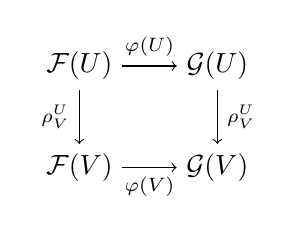
\begin{tikzpicture}
   \matrix (m) [matrix of math nodes, row sep=2em, column sep=2em]
  { \F(U) & \G(U) \\
    \F(V) & \G(V) \\
   };
  \path[->,font=\scriptsize]
  (m-1-1) edge node[auto] {$\varphi(U)$} (m-1-2)
      edge node[auto,swap] {$\rho^U_V$} (m-2-1)
  (m-2-1) edge node[auto,swap] {$\varphi(V)$} (m-2-2)
  (m-1-2) edge node[auto] {$\rho^U_V$} (m-2-2);
\end{tikzpicture}
\end{center}

Sei $f \in \F(U)$. F\"ur alle $V \subseteq U, V \in \mathcal{B}$ sind die Schnitte $\rho^U_V(\varphi(U)(f)) = \varphi(V)(\rho^U_V(f)) \in \G(V)$ festgelegt und bilden eine konsistente Familie in $\G$. Da $\G$ eine Garbe ist, ist $\varphi(U)(f) \in \G(U)$ damit eindeutig bestimmt.

Ist $U' \subseteq U \subseteq X$ offen, dann ist jedes $V \subseteq U', V \in \mathcal{B}$ auch in $U$ enthalten. Es gilt $\rho^{U'}_V(\rho^U_{U'}(\varphi(U)(f))) = \rho^U_V(\varphi(U)(f)) = \varphi(V)(\rho^U_V(f))$, also ist $\rho^U_{U'}(\varphi(U)(f))$ ein Amalgam f\"ur die $\varphi(V)(\rho^U_V(f))$ und es gilt $\rho^U_{U'}(\varphi(U)(f)) = \varphi(U')(\rho^U_ {U'}(f))$. 

\item Hier muss man sich klar machen, dass $\F(U)$ eine (abelsche) Gruppe/ein Ring/ein $R$-Modul ist, falls die $\F'(V)$ es sind und dass die Restriktionsabbildungen in der entsprechenden Kategorie liegen. Auch in b) muss gezeigt werden, dass die $\varphi(U)$ Morphismen aus der richtigen Kategorie sind.
\end{enumerate}

\textit{Anmerkung:} Nat\"urlich h\"atte man bei dieser Aufgabe alles noch ein wenig kategorieller formulieren k\"onnen und vor allem die UAE des inversen Limes mit ins Spiel bringen.
\end{Loes}

%-------------------------- Uebung 2 --------------------------
\newpage
\section{7. Mai 2012}
\setcounter{Aufg}{0}
\setcounter{Loes}{0}

Auf diesem Blatt bezeichne $R$ immer einen kommutativen Ring mit Eins und $k$ einen %algebraisch abgeschlossenen 
K\"orper.

\begin{Aufg}[4 Punkte]
 Beweise die Proposition 1.14 aus der Vorlesung:
Sei $f\colon X\to Y$ stetig, $\mathcal{F}$ eine Garbe auf $X$ und $\G$ eine Garbe auf $Y$.
Dann ist $f^{-1}$ linksadjungiert zu $f_\ast$ in der Kategorie der Garben, d.\,h. es gibt eine nat\"urliche Bijektion 
$$\Hom(f^{-1}\G, \F) \to \Hom(\G, f_\ast \F) \,.$$
\end{Aufg}

 
\begin{Aufg}[4 Punkte]
Zeige das folgende Lemma von Krull:
\begin{enumerate}%[topsep=0cm, parsep=0cm, label=\alph*)]
 \item Sei $S \subseteq R$ ein multiplikatives System und $I \subseteq R$ ein Ideal, das disjunkt zu $S$ ist.
Dann gibt es ein Primideal $\wp \subseteq R$, das $I$ enth\"alt und ebenfalls zu $S$ disjunkt ist.
 \item Es gilt: $$\bigcap_{\stackrel{\wp \textrm{ Primideal in } R}{I \subseteq \wp}} \wp = \sqrt{I}\,.$$
\end{enumerate}
\end{Aufg}

\begin{Aufg}[2 Punkte]
 Zeige:
\begin{enumerate}%[topsep=0cm, parsep=0cm, label=\alph*)]
 \item Jede \textbf{abgeschlossene, nicht leere,} irreduzible Teilmenge von $\Spec R$ hat genau einen generischen Punkt.
 \item Die irreduziblen Komponenten von $\Spec R$ entsprechen bijektiv den minimalen Primidealen in $R$.
\end{enumerate}
\end{Aufg}

\begin{Aufg}[6 Punkte]
 Bestimme $\Spec R$ f\"ur folgende Ringe $R$:
\begin{enumerate}%[topsep=0cm, parsep=0.1cm, label=\alph*)]
 \item $R = \Z/n\!\Z$ f\"ur $n\in \N$.
 \item $R = k[X]/(X^2)$.
 \item $R = k[X]_{(X)} = k[X]_S$ mit $S = k[X]\setminus(X)$.
 \item $R = \C[A]$, die von $A\in \C^{n\times n}$ im Matrizenring $\C^{n\times n}$ erzeugte $\C$-Unteralgebra.
 
 \textit{Hinweis: Hier kann die Lineare Algebra helfen.}
\end{enumerate}
\end{Aufg}

\textbf{Direkter Limes:}

$(I, \le)$ gerichtet $:\Leftrightarrow$ teilgeordnet und jede endliche Teilmenge hat obere Schranke

Gerichtetes System in Kategorie $\mathcal K$ zu $(I, \le)$ ist kovarianter Funktor von $(I, \le)$ nach $\mathcal K$. Der direkte Limes (falls er existiert) zu diesem gerichteten System ist ein $\varinjlim A_i \in \Ob(\mathcal K)$ zusammen mit $\psi_j: A_{j} \to \varinjlim A_i \in \Mor_{\mathcal K}(A_{j}, \varinjlim A_i)$,  sodass:\\
\begin{center}
$j\le k$
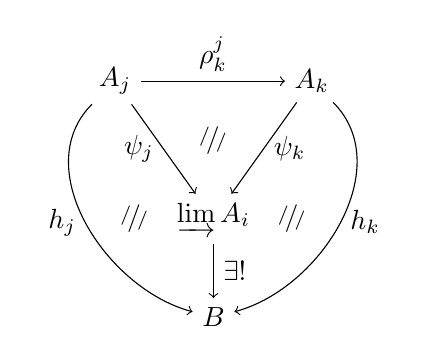
\begin{tikzpicture}[baseline = 0]
	\node (0) at (-1.25, 1.25) {$A_j$};
	\node (1) at (1.25, 1.25) {$A_k$};
	\node (2) at (0, -0.5) {$\varinjlim A_i$};
	\node (3) at (0, -1.75) {$B$};
	\node (4) at (0, 0.5) {$\schraffiert$};
	\node (5) at (-1, -0.5) {$\schraffiert$};
	\node (6) at (1, -0.5) {$\schraffiert$};
	
	\draw [->] (0) -- node[left]{$\psi_j$} (2);
	\draw [->] (1) -- node[right]{$\psi_k$} (2);
	\draw [->] (0) -- node[above]{$\rho_k^j$} (1);
	\draw [->] (2) -- node[right]{$\exists!$} (3);
	
	\draw [->] (0) to [out=225,in=165] node[left]{$h_j$} (3);
	\draw [->] (1) to [out=315,in=15] node[right]{$h_k$} (3);
\end{tikzpicture}
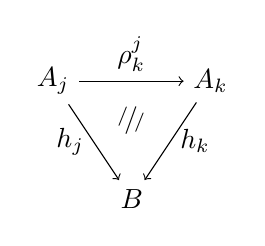
\begin{tikzpicture}[baseline = 0]
	\node (0) at (-1, 0.5) {$A_j$};
	\node (1) at (1, 0.5) {$A_k$};
	\node (2) at (0, -1) {$B$};
	\node (3) at (0, 0) {$\schraffiert$};

	\draw [->] (0) -- node[left]{$h_j$} (2);
	\draw [->] (1) -- node[right]{$h_k$} (2);
	\draw [->] (0) -- node[above]{$\rho_k^j$} (1);
\end{tikzpicture}
\end{center}
$\forall B \in \Ob(\mathcal K)$ zusammen mit $h_{j}: A_{j} \to B $ mit Diagramme kommutieren (siehe oben)\\
$\Rightarrow \exists! f: \varinjlim A_i \to B : f \circ \psi_k = h_k \forall k \in I$

\begin{Loes}
$X, Y$ R\"aume , $f: X \to Y$ stetig, $\calF$ Garbe auf $X$, $\calG$ Garbe auf $Y$ (von abelschen Gruppen)

\textbf{Erinnerung:}\begin{itemize}
\item direkte Bildgarbe: $\forall  V \subseteq Y: f_{*}\calF(V) = \calF(f^{-1} V)$
\item Urbildgarbe: $\forall U\subseteq X: f^{-1} \calG(U) = \varinjlim\limits_{f(U) \subseteq V \in \Off(Y)} \calG(V)$
\end{itemize}
\emph{Zu zeigen:} $f^{-1}$ adjungiert zu $f_{*}$, das hei\ss t es gibt eine in $\calF$ und $\calG$ nat\"urliche Bijektion $\Hom(f^{-1}\calG, \calF) \to \Hom(\calG, f_*\calF)$

Sei $\alpha \in \Hom(f^{-1}\calG, \calF)$\\
$\Rightarrow f_*\alpha : f_*f^{-1}\calG \to f_*\calF$ durch $(f_*\alpha)(V) = \alpha (f^{-1}(V))$ $\leadsto$ es fehlt noch: $\calG \to f_{*}f^{-1}\calG$\\
Sei $V \in \Off(Y)$:
	\[ f_{*}f^{-1}\calG(V) = f^{-1}\calG(f^{-1}(V)) = \varinjlim\limits_{f(f^{-1}(V)) \subseteq W \in \Off(Y)} \calG(W)\]
da $f(f^{-1}(V)) \subseteq V$\\
Zum direkten Limes geh\"ort $\psi(V): \calG(V) \to \varinjlim\limits_{f(f^{-1}(V)) \subseteq W \in \Off(Y)} \calG(W)$.\\
Sei $\beta \in \Hom(\calG, f_*\calF) \Rightarrow f^{-1}\beta: f^{-1}\calG \to f^{-1} f_*\calF$. Sei $U\in \Off(X)$:
	\[f^{1}f_*\calF(U) = \varinjlim\limits_{f(U) \subseteq V \in \Off(Y)} f_*\calF(V) = \varinjlim\limits_{f(U) \subseteq V \in \Off(Y)}\calF(f^{-1}(U)) \]
$f^{-1}\calG(U) = \varinjlim\limits_{f(U) \subseteq V \in \Off(Y)} \calG(V)$\\
Seien $V', V'' \in \Off(Y)$, $f(U) \subseteq V' \subseteq V''$, $\exists! f^{-1}\beta$
\begin{center}
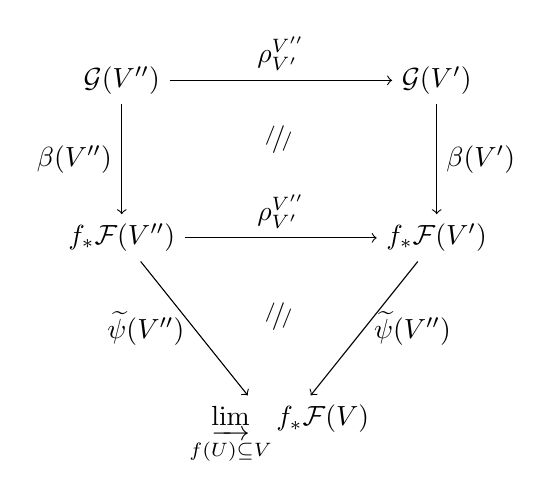
\begin{tikzpicture}[baseline = 0]
	\node (0) at (-2,2) {$\calG(V'')$};
	\node (1) at (2,2) {$\calG(V')$};
	\node (2) at (-2,0) {$f_*\calF(V'')$};
	\node (3) at (2,0) {$f_*\calF(V')$};
	\node (4) at (0,-2.5) {$\varinjlim\limits_{f(U) \subseteq V} f_*\calF(V)$};
	
	\node at (0, 1.25) {$\schraffiert$};
	\node at (0, -1) {$\schraffiert$};
	
	\draw[->] (0) -- node[above]{$\rho_{V'}^{V''}$} (1);
	\draw[->] (2) -- node[above]{$\rho_{V'}^{V''}$} (3);
	
	\draw[->] (0) -- node[left]{$\beta(V'')$} (2);
	\draw[->] (1) -- node[right]{$\beta(V')$} (3);
	
	\draw[->] (2) -- node[left]{$\widetilde \psi(V'')$}(4);
	\draw[->] (3) -- node[right]{$\widetilde \psi(V'')$}(4);
\end{tikzpicture}
$\Longrightarrow$
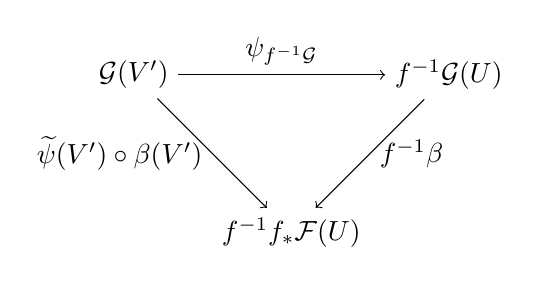
\begin{tikzpicture}[baseline = 0]
	\node (0) at (-2, 1) {$\calG(V')$};
	\node (1) at (2, 1) {$f^{-1}\calG(U)$};
	\node (2) at (0, -1) {$f^{-1}f_*\calF(U)$};

	\draw [->] (0) -- node[left]{$\widetilde \psi (V') \circ \beta(V')$} (2);
	\draw [->] (1) -- node[right]{$f^{-1}\beta$} (2);
	\draw [->] (0) -- node[above]{$\psi_{f^{-1}\calG}$} (1);
\end{tikzpicture}

\end{center}
Es fehlt noch: $\varphi_\calF: f^{-1}f_*\calF \to \calF$\\
Seien $V',V''$ wie eben. Dann: $U\subseteq f^{-1}(V') \subseteq f^{-1}(V'')$
\begin{center}
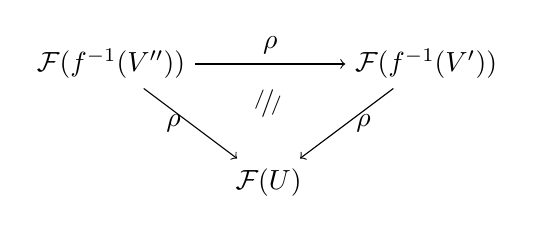
\begin{tikzpicture}[baseline = 0]
	\node (0) at (-2, 0.5) {$\calF(f^{-1}(V''))$};
	\node (1) at (2, 0.5) {$\calF(f^{-1}(V'))$};
	\node (2) at (0, -1) {$\calF(U)$};
	\node (3) at (0, 0) {$\schraffiert$};

	\draw [->] (0) -- node[left]{$\rho$} (2);
	\draw [->] (1) -- node[right]{$\rho$} (2);
	\draw [->] (0) -- node[above]{$\rho$} (1);
\end{tikzpicture}
\end{center}
$\Rightarrow \exists! \varphi_\calF(U): f^{-1}f_*\calF(U): \varphi_\calF \circ \tilde \psi = \rho$\\
Definiere:
\begin{equation*}\begin{array}{rlcccl}
	T_1:& \Hom(f^{-1}\calG, \calF) &\ni &\alpha &\mapsto &f_* \alpha \circ \psi_\calG \in \Hom(\calG, f_*\calF)\\
	T_2:& \Hom(\calG, f_*\calF) &\ni &\beta &\mapsto & \textcolor{red}{\text{[FEHLT]}}
\end{array}\end{equation*}
Sei $\alpha \in \Hom(f^{-1}\calG, \calF)$, $U\in \Off(X)$. Sei dazu $V\in \Off(Y)$ mit $f(U)\subseteq V$, also $U\subseteq f^{-1}(f(U)) \subseteq f^{-1}(V)$.
\begin{center}\begin{tikzpicture}
	\node (0) at (1,0) {$f^{-1}f_*\calF(U)$};
	\node (1) at (-4,0) {$\calF(f^{-1}(V)) = f_* \calF(V)$};
	
	\node (2) at (-4,3) {$f^{-1}\calG(f^{-1}(V)) = f_*f^{-1}\calG(V)$};
	\node (3) at (2,3) {$\calG(V)$};
	\node (4) at (7,3) {$f^{-1}\calG(U)$};
	
	\node (5) at (-1,-3) {$\calF(U)$};
	
	\node at (1.5,1.5) {$\schraffiert$};
	\node at (-2.5,1.5) {$\schraffiert$};
	\node at (1.5,4.5) {$\schraffiert$};
	\node at (-2,-1.5) {$\schraffiert$};
	\node at (4.5,0) {$\schraffiert$};
	
	\draw[->] (1) -- node[below]{$\tilde \psi(V)$} (0);
	\draw[->] (2) -- node[left]{$\alpha(f^{-1}(V))=f_*\alpha(V)$} (1);
	\draw[->] (3) -- node[above]{$\psi_\calG(V)$}(2);
	\draw[->] (3) -- node[above]{$\psi_{f^{-1}\calG}(V)$} (4);
	\draw[->, dashed] (3) -- (1);
	\draw[->, dashed] (4) -- node[right]{$f^{-1}(f_*\alpha \circ \psi_\calG)(U)$} (0);
	\draw[->] (0) -- node[right]{$\varphi_\calF(U)$} (5);
	\draw[->] (1) to [out=270,in=180] node[left]{$\rho_U^{f^{-1}(V)}$} (5);
	\draw[->] (2) to [out=45,in=135] node[above]{$\rho_U^{f^{-1}}(V)$} (4);
	\draw[->] (4) to [out=315,in=0] node[right]{$\hat \alpha(U)$}(5);
\end{tikzpicture}\end{center}
Zu zeigen: $\hat \alpha = \alpha$
\end{Loes}

\begin{Loes}
\begin{enumerate}%[topsep=0cm, parsep=2mm, label=\alph*)]
  \item Betrachte den kanonischen Ringhomomorphismus $\varphi\colon R \to R_S$. Sei $I'=\left(\varphi(I)\right)$ das von $\varphi(I)$ erzeugte Ideal in $R_S$, also $I'=\{\frac{f}{a}\in R_S\mid f\in I,\ a\in S\}$.

    Zun\"achst \"uberlegen wir uns, dass $I'\neq R_S$, also $1\notin I'$. Denn w\"are $1\in I'$, dann g\"abe es ein $f\in I$ und ein $a\in S$
    mit $1=\frac{f}{a}$ in $R_S$, d.h. es g\"abe ein
    \[s\in S\text{ mit }s(f-a)=0.\] 
    Dann w\"are $sf=sa$ sowohl in $I$ als auch in $S$ -- ein Widerspruch zur Disjunktheit!

    Somit ist $I'$ ein echtes Ideal und damit in einem maximalen Ideal $\mathfrak{m}'$ enthalten. Dann ist $\mathfrak{p}:=\varphi^{-1}(\mathfrak{m}')$ ein
    Primideal, enth\"alt $I$ und hat leeren Schnitt mit $S$, denn sonst w\"are f\"ur $s\in S\cap \mathfrak{p}$ das Bild $\varphi(s) \in \mathfrak{m}'$ eine Einheit in $R_S$.
  \item \begin{itemize}
         \item["`$\supseteq$"'] Ist $f \in \sqrt{I}$, so existiert ein $n \in \N$ mit $f^n \in I$. Folglich gilt f\"ur alle $\mathfrak{p} \in \Spec R$ mit $I \subseteq \mathfrak{p}$, dass $f^n \in \mathfrak{p}$, also auch $f \in \mathfrak{p}$. 
         \item["`$\subseteq$"'] Sei $a\in R\setminus\!\sqrt{I}$ und $S:=\{a^n\mid n\in\N_0\}$. Dann ist $S$ ein multiplikatives System und $I\cap S=\emptyset$. Nach a) gibt es dann ein Primideal $\mathfrak{p}$ mit $\mathfrak{p} \supseteq I$ und $\mathfrak{p} \cap S=\emptyset$. Damit liegt $a$ nicht im Schnitt \"uber alle Primideale, die $I$ enthalten.
        \end{itemize}
\end{enumerate}
\end{Loes}

\begin{Loes}
$R$ kommutativer Ring mit Eins.
\begin{enumerate}[a)]
\item
	$V \ne \emptyset$, abgeschlossen, irreduzibel, $V \subseteq \Spec R$\\
	$\Rightarrow \underbrace{V = V(I)}_{\{\p \in \Spec R | I \subseteq \p\}}$, $I$ Primideal\\
	$\Rightarrow \overline{\{I\}} = V(I(\{I\})) = V(I) = V$\\
	Seien $\p,\q \in \Spec R$ mit $\overline{\{\p\}} = \overline{\{\q\}}$\\
	$\q \in \overline{\{\p\}} = V(\p) = \{ \tilde \p \in \Spec R | \p \subseteq \tilde \p \} \Rightarrow \q \subseteq \p$\\
	Analog $\q \subseteq \p \Rightarrow \p = \q$
\item
	Seien $\p, \q \in \Spec R$\\
	$\p \subseteq \q\Leftrightarrow \q \in \overline{\{\p\}} \Leftrightarrow \overline{\{\q\}} \subseteq \overline{\{\p\}}$
\end{enumerate}\end{Loes}

\begin{Loes}
$\Spec: \underline{\text{Ringe}} \to \underline{\text{Top.}}$ kontravarianter Funktor, $\alpha: R \to R'$, $\Spec(\alpha):\left\{\begin{array}{ccc}\Spec R' \to \Spec R \\ \p \mapsto \alpha^{-1}(\p)\end{array}\right.$\\
Sei $R$ Ring, $I\subseteq R$ ein Ideal und $\pi: R \twoheadrightarrow R/I$ die kanonische Projektion, dann ist $\Spec \pi \colon \Spec R/I \hookrightarrow \Spec R$ injektiv.
	\[ \Bild(\Spec \pi) = \{\p \in \Spec R | I \subseteq \p\} \]
\begin{enumerate}[a)]
\item
	$R= \FakRaum{\Z}{n\Z}$, $I:=n\Z$, $\pi: \Z \to \FakRaum{\Z}{n\Z}$, $\Bild(\Spec \pi) = \{(p) \in \Spec \Z | p \in \IP, p|n\}$, $x,y\in \FakRaum{\Z}{n\Z}: D(x) \subseteq D(y) \Leftrightarrow \exists z \in \FakRaum{\Z}{n\Z}, m \in \N: x^m = z\cdot y$\\
	\textcolor{gray}{$\left( x \in \FakRaum{\Z}{n\Z} , D(x) = \p \in \Spec R | x\in \p \right)$}\\
	$\rho_{D(x)}^{D(y)}: R_y \to R_x, \frac{a}{y^k}\mapsto \frac{a\cdot z^k}{x^{m\cdot k}}$

 \item Es gilt $\Spec(k[X]) = \{(0)\} \cup \{(f) \mid f \in k[X] \textrm { irreduzibel}\}$.
 Sei $R = k[X]/(X^2)$, $I \coloneqq (X^2)$ und $\pi\colon k[X] \twoheadrightarrow k[X] / I$. Dann ist 
 $$\Bild(\Spec \pi) = \{(f) \in \Spec k[X]/(X^2) \mid f \in k[X] \textrm{ irreduzibel}, (X^2) \subseteq (f) \} = \{(X)\}$$ und somit
 $Y \coloneqq \Spec R = \{(X)\}$ einelementig. Die Strukturgarbe ist dann offensichtlich:
 $$\calO_Y(Y)=R \stackrel{\rho^Y_\emptyset \textrm{ eindeutig}}{\longrightarrow} \{p\} = \calO_Y(\emptyset)$$ 
 
 \item Nun sei $R = k[X]_{(X)} = k[X]_S$ mit $S= k[X] \setminus (X)$. Der Ring ist als Teilring von $k(X)$ nullteilerfrei und somit ist $(0)$ ein Primideal. Au\ss erdem ist der Ring lokal, mit maximalem Ideal $\mathfrak{m} = R \setminus R^{\times} = (\frac{X}{1})$. Sei nun $\emptyset \neq \mathfrak{p} \in \Spec R$ und $f \in \mathfrak{p}$. Dann schreiben wir $f = {\frac{X}{1}}^e \cdot \frac{a}{b}$ mit $a \in k[X], b \in k[X] \setminus (X), X \nmid a$. Dann ist $a \in S$ und $\frac{a}{b}$ somit offensichtlich invertierbar, also gilt $\frac{X}{1}^e \in \mathfrak{p}$. Da $\mathfrak{p}$ prim ist, ist $\frac{X}{1} \in \mathfrak{p}$ und wegen $\mathfrak{p} \subseteq (\frac{X}{1})$ folgt $\mathfrak{p} = (\frac{X}{1})$. Folglich besteht das Spektrum von $R$ aus genau zwei Punkten: $Y \coloneqq \Spec k[X]_{(X)} = \{(0), (\frac{X}{1})\}$. Die offenen Mengen sind $\emptyset, D(\frac{X}{1}) = \{(0)\}$ und $Y$. Auch hier ist die Strukturgarbe leicht anzugeben:
 
 \begin{center}
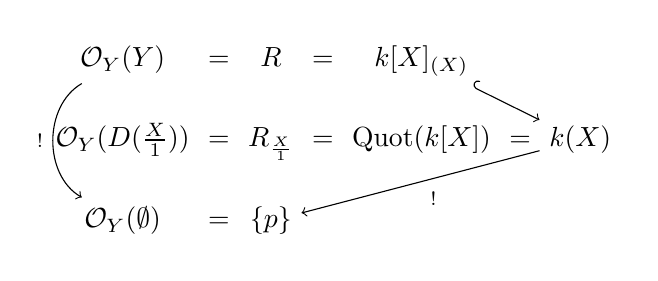
\begin{tikzpicture}
   \matrix (m) [matrix of math nodes, row sep=1em, column sep=0em]
	{ \calO_Y(Y) & = & R & = & k[X]_{(X)}\\
	  \calO_Y(D(\frac{X}{1})) & = & R_{\frac{X}{1}} & = & \Quot(k[X]) & = & k(X)\\
	  \calO_Y(\emptyset) &=& \{p\}\\
	 };
  \path[right hook->,font=\scriptsize]
	(m-1-5) edge (m-2-7);
  \path[->, font=\scriptsize]
	(m-1-1) edge [bend right=60] node[auto,swap] {!} (m-3-1)
	(m-2-7) edge node[auto] {!} (m-3-3);
\end{tikzpicture}
\end{center}
 
 
 \item Wir betrachten den Einsetzungshomomorphismus $\Psi_A: \C[X] \twoheadrightarrow \C[A]$. Der Kern von $\Psi_A$ ist $(\mathfrak{m}_A)$, wobei $\mathfrak{m}_A = \prod_{i=1}^e (X-\lambda_i)^{r_i}$ das Minimalpolynom von $A$ ist, mit den Eigenwerten $\lambda_i$ von $A$. Nach dem Homomorphiesatz ist $\C[A] \cong \C[X]/(\mathfrak{m}_A)$. Unsere  Vor\"uberlegungen liefern dann, genau wie in a) und b), 
 $$\Bild(\Spec \Psi_a) = \{ \mathfrak{q} \in \Spec \C[X] \mid (\mathfrak{m}_A) \subseteq \mathfrak{q} \} = \{(X- \lambda_i) \mid \lambda_i \textrm{ ist EW von } A \}$$
 und somit $\Spec \C[A] = \{(A- \lambda_i) \mid \lambda_i \textrm{ ist EW von } A\}$.
\end{enumerate}

\end{Loes}

%-------------------------- Uebung 3 --------------------------
\newpage
\section{15. Mai 2012}
\setcounter{Aufg}{0}
\setcounter{Loes}{0}

Auf diesem Blatt bezeichne $R$ immer einen kommutativen Ring mit Eins.

\begin{Aufg}[4 Punkte]\label{a3.1}
 Sei $\left(X, \mathcal{O}_X \right)$ ein Schema und $(\Spec R,\calO_{\Spec R})$ ein affines Schema.
Zeige, dass die Zuordnung 
$$\begin{array}{rcl}
   \Mor(X, \Spec R) &\to& \Hom(R, \mathcal{O}_X(X))\,,\\
   (\varphi, \varphi^\sharp) &\mapsto& \varphi^\sharp(\Spec R)
  \end{array}
$$ 
bijektiv ist.
\end{Aufg}


\begin{Aufg}[6 Punkte]
 \begin{enumerate}%[topsep=0cm, parsep=0cm, label=\alph*)]
 \item Zeige, dass $(\Spec \Z, \calO_{\Spec \Z})$ ein terminales Objekt in der Kategorie der affinen Schemata ist, dass es also zu jedem affinen Schema $(\Spec R,\calO_{\Spec R})$ genau einen Morphismus $(\varphi, \varphi^\sharp)$ von lokal geringten R\"aumen nach $(\Spec \Z, \calO_{\Spec \Z})$ gibt. 
  \item Finde jeweils einen Ring $R$, so dass der Morphismus $(\varphi, \varphi^\sharp)$ aus a)
 \begin{itemize}
  \item genau einen Punkt als Bild hat,
  \item genau zwei Punkte als Bild hat,
  \item unendlich viele Punkte als Bild hat, aber nicht surjektiv ist,
  \item surjektiv ist.
 \end{itemize}
\end{enumerate}
\end{Aufg}


\begin{Aufg}[4 Punkte]
Zeige:
\begin{enumerate}%[topsep=0cm, parsep=0cm, label=\alph*)]
 \item Ein Element $e\in R$ ist genau dann idempotent (d.h. es gilt $e^2 = e$), wenn $1-e$ idempotent ist.
 \item Gibt es in $R$ zwei Elemente $e_1$, $e_2 \not\in R^\times$, so dass $e_1+e_2 =1$ und $e_1\cdot e_2$ nilpotent ist, so enth\"alt $R$ mindestens drei idempotente Elemente.
 
 \textit{Hinweis: Betrachte das Ideal $I_n = (e_1^n, e_2^n)$ f\"ur $n\in \N$.}
 \item $\Spec R$ ist genau dann zusammenh\"angend, wenn $R$ h\"ochstens zwei idempotente Elemente enth\"alt.
 \item Gib einen Ring $R$ an, sodass $\Spec R$ nicht zusammenh\"angend ist.
\end{enumerate}
\end{Aufg}

\begin{Loes}
$(X, \calO_X)$ Schema, $(\Spec R, \calO_{\Spec R})$ affines Schema\\
\emph{Zu zeigen:} $\begin{array}{rcl} \Mor(X, \Spec R) &\to& \Hom(R, \calO_X(X))\\ (\varphi, \varphi^\#) &\mapsto& \varphi^\# (\Spec R) \end{array}$ ist bijektiv

Konstruiere die Umkehrabbildung. Sei $\Phi: R\to \calO_X(X)$ Ringhomomorphismus. Konstruiere $\varphi: X\to \Spec R$ stetig (bez\"uglich Zariski-Topologie).\\
Sei $p \in X$, $R \xrightarrow{\Phi} \calO_X(X) \xrightarrow{\Psi_X} \calO_{X,p} = \varinjlim\limits_{p\in U \in \Off(X)} \calO_X(U)$\\
$\calO_{X,p}$ ist lokaler Ring mit maximalem Ideal $m_p$. Setze $\varphi(p):=(\Psi_X \circ \Phi)^{-1}(m_p)$.

\emph{Behauptung:} $\varphi$ ist stetig\\
\emph{denn:} Es reicht das f\"ur Basismengen zu \"uberpr\"ufen $\leadsto$ auf affinen Teilen reicht.

Sei $\Spec S \subseteq X$, $p\in S\Spec S$
\begin{center}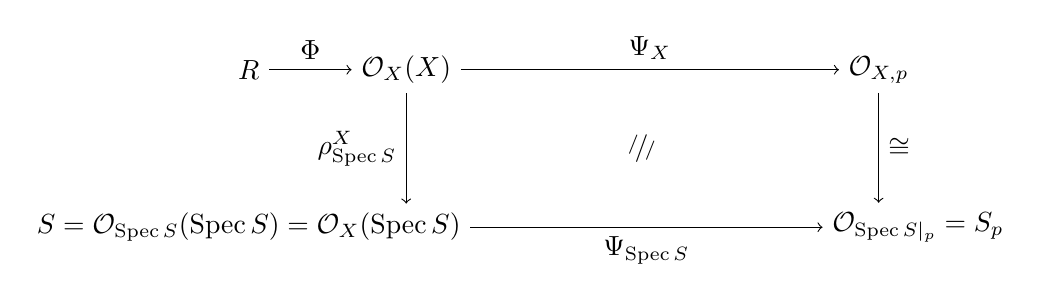
\begin{tikzpicture}
	\node (0) at (-5, 1) {$R$};
	\node (1) at (-3, 1) {$\calO_X(X)$};
	\node (2) at (3, 1) {$\calO_{X, p}$};
	\node (3') at (-3, -1) {\textcolor{white}{$\calO_X(\Spec S)$}}; %auf diesen Knoten wird der Pfeil gezeichnet
	\node (3) at (-5, -1) {$S = \calO_{\Spec S}(\Spec S) = \calO_X(\Spec S)$}; %dieser Knoten wird zu sehen sein
	\node (4) at (3, -1) {\textcolor{white}{$\calO_{\Spec S|_p}$}};
	\node (4') at (3.5, -1) {$\calO_{\Spec S|_p} = S_p$};
	
	\node at (0, 0) {$\schraffiert$};
	
	\draw[->] (0) -- node[above]{$\Phi$} (1);
	\draw[->] (1) -- node[above]{$\Psi_X$} (2);
	\draw[->] (3) -- node[below]{$\Psi_{\Spec S}$} (4');
	\draw[->] (1) -- node[left]{$\rho_{\Spec S}^X$} (3');
	\draw[->] (2) -- node[right]{$\cong$} (4);
\end{tikzpicture}\end{center}
$(\Psi_X \circ \Phi)^{-1}(m_p) = (\Psi_{\Spec S} \circ \rho_{\Spec S}^X \circ \Phi)^{-1} (p) = \Phi^{-1} (\rho_{\Spec S}^X (p))$ $\Rightarrow $ auf allen affinen Teilen gilt: $\varphi|_{\Spec S}(p) = \Phi^{-1}(p)$ $\leadsto$ nach Bemerkung \ref{2.4} stetig.

Konstruiere Garbenmorphismus $\varphi^\#: \calO_{\Spec R} \to \varphi_*\calO_X$. Sei $f\in R$, $D(f) = \{p \in \Spec R | f\notin p\} \subseteq \Spec R$.
\begin{center}(*)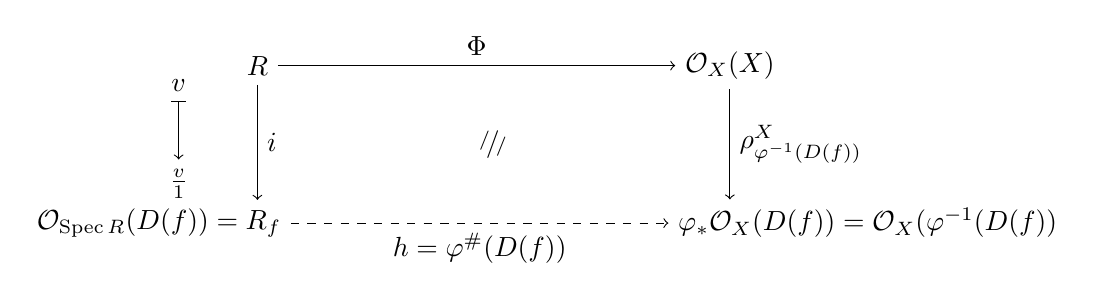
\begin{tikzpicture}[baseline=0]
	\node (0) at (-3, 1) {$R$};
	\node (1) at (3, 1) {$\calO_X(X)$};
	\node (2') at (-3, -1) {\textcolor{white}{$R_f$}};
	\node (2) at (-4.25, -1) {$\calO_{\Spec R}(D(f))=R_f$};
	\node (3') at (3, -1) {\textcolor{white}{$\varphi_*\calO_X(D(f))$}};
	\node (3) at (4.75, -1) {$\varphi_*\calO_X(D(f)) = \calO_X(\varphi^{-1}(D(f))$};

	\node (4) at (-4, 0.75) {$v$};
	\node (5) at (-4, -0.5) {$\frac{v}{1}$};
	
	\node at (0, 0) {$\schraffiert$};
	
	\draw[->] (0) -- node[above]{$\Phi$} (1);
	\draw[->] (0) -- node[right]{$i$} (2');
	\draw[->] (1) -- node[right]{$\rho_{\varphi^{-1}(D(f))}^X$} (3');
	\draw[->, dashed] (2) -- node[below]{$h = \varphi^\#(D(f))$} (3);
	\draw[|->] (4) -- (5);

\end{tikzpicture}
\\ \ \\$S=\{f^n|n\in \N\}$\end{center}
\emph{UAE Lokalisierung:} Falls $(\rho \circ \Phi)(S) \subseteq \varphi_*\calO_X(D(f))^\times \Rightarrow \exists! h : R_f \to \varphi_*\calO_*(D(f))$\\
$\rho \circ \Phi = h \circ i$

$\varphi^{-1}(D(f)) = \{q \in X | \varphi(q) \in D(f)\} = \{q \in X | f \notin \varphi(q)\}$\\
F\"ur $q \in \Spec S \subseteq X$ gilt:
	\[f \notin \varphi(q) = \Phi^{-1}((\rho_{\Spec S}^X)^{-1}(q)) \Leftrightarrow \rho_{\Spec S}^X (\Phi(f)) \in q \Leftrightarrow q \in D(\rho_{\Spec S}^X(\Phi(f))) = S_{\rho_{\Spec S}^X (\Phi (f))} \]
$\Rightarrow \rho_{\varphi^{-1}(D(f)) \cap \Spec S}^X (\Phi(f))$ ist invertierbar.\\
$\calO_X$ Garbe $\Rightarrow $ Inverse von $\varphi(\Phi(f))$ setzen sich zu \quot{globalem} Inversen zusammen.\\
$\xRightarrow{\text{UAE}} \exists! \varphi^\#(D(f)) : \calO_{\Spec R}(D(f)) \to \varphi_*\calO_X(D(f))$ mit (*) $\leadsto$ passt auch auf $D(f) \cap D(g)$ zusammen.\\
$\xRightarrow[\text{Aufgabe 3}]{\text{Blatt 1}}$ eindeutige Forsetzung Garbenmorphismus $\varphi^\#: \calO_{\Spec R} \to \varphi_*\calO_X$

\emph{Zeige:} $\varphi^\#$ induziert lokale Ringhomomorphismen auf Halmen.

F\"ur $q \in \Spec S \subseteq X$ gilt $\calO_{X,q} = \calO_{\Spec S, q} = S_q$. Setze $p:= \varphi(q) \subseteq \Spec R$.\\
$\Rightarrow \varphi_p^\#(p): \left\{ \begin{array}{rcl} \calO_{\Spec R, p} = R_p &\to& S_q \\ \frac{a}{b} &\mapsto& \frac{\rho_{Spec S}^X (\Phi(a))}{\rho_{Spec S}^X (\Phi(b))} \end{array}\right.$

\emph{Noch zu zeigen:} $f^\#(\Spec R) = \Phi$

$\Spec R = D(1) \checkmark$\\
$(\varphi, \varphi^\#) \to \varphi^\#(\Spec R) \to (\varphi', (\varphi^{\#})' )$ ist Identit\"at.
\end{Loes}

\begin{Loes}\begin{enumerate}[a)]
\item
	$(\Spec \Z, \calO_{\Spec \Z})$ ist terminales Objekt in der Kategorie der Schemata (\quot{affin} ist \"uberfl\"ussig). Ist $(X, \calO_X)$ Schema, $\exists! \Phi:\left\{\begin{array}{rcl} \Z &\to& \calO_X(X)\\ 1 &\mapsto& 1\end{array}\right.$ Ringhomomorphismus $\xRightarrow{\text{Aufgabe 1}} \exists! (\varphi, \varphi^\#): X \to \Spec \Z$ Schemamorphismus
\item
	\begin{description}[\setlabelstyle{\itshape}]
	\item[Genau ein Punkt im Bild:]
		$R=K$ K\"orper $\Rightarrow \Spec K= \{(0)\}$\\
		$\Phi:\left\{ \begin{array}{rcl} \Z &\to& K \\ 1 &\mapsto& 1 \end{array}\right.$, $\Phi^{-1}((0)) = (p) \in \Spec \Z$, $p = \chara K$, $\varphi((0)) = (p)$\\
		$\varphi_p^\#: \left\{\begin{array}{rcl} \calO_{\Spec \Z, p} \cong \Z_p &\to& \calO_{\Spec K, (0)} = K_{(0)} = k \\ \frac{f}{g} &\mapsto& \FakRaum{\Phi(f)}{\Phi(g)}\end{array}\right.$
	\item[Genau zwei Punkte:]
		$R=\Z_{(p)}$, $\Spec R = \{ (0), (p)\}$\\
		$\Phi: \left\{\begin{array}{rcl} \Z &\to& \Z(p) \\ 1 &\mapsto& \frac{1}{1}\end{array}\right.$\\
		$\begin{array}{l} \varphi((0)) = \Phi^{-1}((0)) = (0) \\ \varphi((p)) = (p)\end{array} \Rightarrow $ Bild zweielementig
	\item[unendliches Bild, nicht surjektiv:]
		Bemerkung: Ist $R$ kommutativer Ring mit $1$, $S\subseteq R$ multiplikatives System, $\Phi: R \to R_S$, $\Spec \Phi: \Spec R_S \to \Spec R$ $\Rightarrow \Bild(\Spec \Phi) = \{p \in \Spec R | p \cap S = \emptyset\}$. $\Spec \Phi$ ist Bijektion auf das Bild (sogar Hom\"oomorphismus).
		
		$R= \Z_n, n\in \N$\\
		$\Rightarrow \Bild(\Spec \Phi) = \{(p) \in \Spec \Z |p \in \IP, p \nmid n\}$\\
		$\Rightarrow \Bild(\Spec \Phi) \ne \Spec \Z$ f\"ur $n \ge 2$
	\item[surjektiv:]$\id: \Z \to \Z$\\
		$\id: \Spec\Z \to \Spec\Z$
	\end{description}
\end{enumerate}\end{Loes}

\begin{Loes}\begin{enumerate}[a)]
\item
	Sei $e^2 = e$ dann ist $(1-e)^2 = 1 -2e + e^2 = 1-e$. Mit $1-(1-e) = e$ folgt die andere Richtung.
\item
	Seien $e_1,e_2 \in R\setminus R^{\times}$ mit $e_1 + e_2 =1$, $e_1e_2$ nilpotent $\Rightarrow R$ enth\"alt mindestens drei idempotente Elemente.
	
	$0$, $1$ sind idempotent\\
	$I_n = (e_1^n, e_2^n)$, $n\in \N$\begin{enumerate}[\textbullet]
	\item
		$\sqrt{I_n} = R$, denn: $e_1, e_2 \in \sqrt{I_n} \Rightarrow 1= e_1 + e_2 \in \sqrt{I_n}$
	\item
		$I_n = R$, denn sonst: $I_n \subseteq m$, $m$ maximales Ideal $\Rightarrow \sqrt{I_n} \subseteq m$ $\lightning$ zu $\sqrt{I_n} = R$
	\end{enumerate}
	$\Rightarrow \forall n \in \N \exists  \alpha_n, \beta_n \in R: \alpha_n e_1^n + \beta_n e_2^n = 1$\\
	$e_1e_2$ nilpotent $\Rightarrow \exists k \in \N: (e_1e_2)^k = 0$\\
	$x = \alpha_ke_1^k = 1 - \beta_ke_2^k$ ist idempotent\\
	$x^2 = \alpha_ke_1^k (1- \beta_ke_2^k) = \alpha_k e_1^k - \alpha_k \beta_k (\underbrace{e_1e_2}_{=0})^k = x$\\
	Es bleibt zu zeigen, dass $x$ weder $1$ noch $0$ ist. Wäre $x=0$, so wäre $\beta e_2^k = 1$, also $e_2 \in R^\times$, was im Widerspruch zur gegenteiligen Voraussetzung steht. Analog folgt aus $x = \alpha e_1^k = 1$, dass $e_1 \in R^\times$.
  
  \item Sei zunächst $\Spec R$ zusammenhängend. Wir nehmen an, es gäbe drei verschiedenen idempotente Elemente, $0,1$ und $x$. Nach a) ist dann auch $1-x$ idempotent. Setze $V_1 = V(x)$ und $V_2 = V(1-x)$. Die Mengen sind abgeschlossen (klar) und nichtleer: 
  Wäre $V_1 = \emptyset$, so wäre $x$ in keinem echten Ideal enthalten, also invertierbar und wegen $x^2 = x$ gleich $1$. Genauso folgt aus $V_2 = \emptyset$, dass $1-x\in R^{\times}$ und mit $(1-x)^2 = (1-x)$, dass $x = 0$.

  Angenommen es gäbe ein $\p \in V(x)\cap V(1-x)$. Für dieses gälte $x$ und $1-x \in \p$, also auch $1\in \p$, ein Widerspruch. Andererseits ist $V(x)\cup V(1-x) = V(x(1-x))= V(0) = \Spec(R)$. Damit haben wir eine disjunkte Zerlegung von $\Spec(R)$ in abgeschlossene, nichtleere Teilmengen gefunden, im Widerspruch zur Voraussetzung. Also gibt es höchstens zwei idempotente Elemente in $R$.

  Nun sei $\Spec(R)$ nicht zusammenhängend. Wir finden ein drittes idempotentes Element. Sei $\Spec(R) = V_1 \cup V_2$ eine Zerlegung in abgeschlossene, disjunkte, nichtleere Teilmengen. Es ist $V_1 = V(I_1)$ und $V_2 = V(I_2)$, für Ideale $I_1, I_2 \subseteq R$. Da ihr Durchschnitt $V(I_1) \cap V(I_2) = V(I_1+I_2) = \emptyset = V(1)$ ist, folgt $I_1+I_2 = R$, und es gibt $e_1\in I_1$, $e_2\in I_2$ mit $e_1+e_2 = 1$. Andererseits ist weder $e_1$ noch $e_2$ eine Einheit, denn beide Verschwindungsmengen sind nichtleer. Außerdem ist $V(I_1)\cup V(I_2) = V(I_1\cdot I_2) = \Spec(R) = V(\sqrt{0})$ gleich der Verschwindungsmenge des Nilradikals. Also folgt $I_1\cdot I_2 \subseteq \sqrt{0}$ und damit ist $e_1e_2$ nilpotent.

  \item Es sei $R$ ein beliebiger Ring mit $1$ und $S= R\times R$ mit der komponentenweisen Verknüpfung. Dann ist $(1,0)$ ein idempotentes Element in $S$, dass weder $(0,0)$ noch $(1,1)$ ist. Also ist $\Spec S$ nach c) nicht zusammenhängend.
\end{enumerate}\end{Loes}

%-------------------------- Uebung 4 --------------------------
\newpage
\section{22. Mai 2012}
\setcounter{Aufg}{0}
\setcounter{Loes}{0}

\begin{Aufg}[4 Punkte]
 Seien $R$, $S$ Ringe, $X\coloneqq\textup{Spec}(R)$, $Y\coloneqq\textup{Spec}(S)$ sowie $\varphi \colon R \to S$ ein Ringhomomorphismus und $g \colon Y \to X$ der von $\varphi$ induzierte Schemamorphismus. Zeige:
\begin{enumerate}%[topsep=0cm, parsep=0cm, label=\alph*)]
\item Ein Element $f \in R$ ist genau dann nilpotent, wenn $D(f)$ leer ist.
\item Der Ringhomomorphismus $\varphi$ ist genau dann injektiv, wenn der induzierte Morphismus $g^\sharp \colon \mathcal{O}_X \to g_* \mathcal{O}_Y$ injektiv ist. Ist das der Fall, so ist $g$ dominant, d.h. $g(Y)$ ist dicht in $X$.
\item Ist $\varphi$ surjektiv, so ist $g$ ein Homöomorphismus von $Y$ auf eine abgeschlossene Teilmenge von $X$ und $g^\sharp \colon \mathcal{O}_X \rightarrow g_* \mathcal{O}_Y$ ist surjektiv.
\end{enumerate}
\end{Aufg}

\begin{Aufg}[4 Punkte]
 Finde einen Ring $R$ und eine Idealgarbe $\mathcal{I}$ auf $\Spec(R)$, die nicht quasikohärent ist (und beweise, dass du solche $R$ und $\mathcal{I}$ gefunden hast).

\textit{Hinweis: Diskrete Bewertungsringe können helfen.}
\end{Aufg}

\begin{Aufg}[4 Punkte]
 Beweise die Proposition 4.5 aus der Vorlesung:

Eine Idealgarbe $\mathcal{I}$ auf einem Schema $X$ ist genau dann quasikohärent, wenn es eine offene Überdeckung $(U_i)_{i \in M}$ von $X$ durch affine Schemata $U_i$ gibt, so dass $\mathcal{I}|_{U_i}$ für jedes $i \in M$ quasikohärent ist.
\end{Aufg}

\begin{Loes}

\end{Loes}

\begin{Loes}

\end{Loes}

\begin{Loes}

\end{Loes}

%-------------------------- Uebung 5 --------------------------
\newpage
\section{29. Mai 2012}
\setcounter{Aufg}{0}
\setcounter{Loes}{0}

%-------------------------- Uebung 6 --------------------------
\newpage
\section{5. Juni 2012}
\setcounter{Aufg}{0}
\setcounter{Loes}{0}

%-------------------------- Uebung 7 --------------------------
\newpage
\section{12. Juni 2012}
\setcounter{Aufg}{0}
\setcounter{Loes}{0}

%-------------------------- Uebung 8 --------------------------
\newpage
\section{19. Juni 2012}
\setcounter{Aufg}{0}
\setcounter{Loes}{0}

%-------------------------- Uebung 9 --------------------------
\newpage
\section{26. Juni 2012}
\setcounter{Aufg}{0}
\setcounter{Loes}{0}

%-------------------------- Uebung 10 --------------------------
\newpage
\section{3. Juli 2012}
\setcounter{Aufg}{0}
\setcounter{Loes}{0}

%-------------------------- Uebung 11 --------------------------
\newpage
\section{10. Juli 2012}
\setcounter{Aufg}{0}
\setcounter{Loes}{0}

%-------------------------- Uebung 12 --------------------------
\newpage
\section{17. Juli 2012}
\setcounter{Aufg}{0}
\setcounter{Loes}{0}

%-------------------------- Uebung 13 --------------------------
\newpage
\section{24. Juli 2012}
\setcounter{Aufg}{0}
\setcounter{Loes}{0}

%-_-_-_-_-_-_-_-_-_-_-_-_-_-_ Gaestebuch -_-_-_-_-_-_-_-_-_-_-_-_-_-_-_-_


\chapter{G\"astebuch}
Hier kann jeder, der g\"o\ss ere \"Anderungen oder Korrekturen am Skript vorgenommen hat, seinen Namen und einen Kommentar hinterlassen. Kleinigkeiten wie Rechtschreibfehler m\"ussen nicht unbedingt sein (und bei meinen Tippfehlern w\"are das G\"astebuch gr\"o\ss er als das Skript), aber ein korrigierter Satz, ein vervollst\"andigter Beweis, solche Sachen, einfach damit jemand der eine \"altere Version des Skriptes hat schnell den Unterschied finden kann. Oder hinterlasst einfach ein Paar nette Worte :-)

Zum Schreiben im G\"astebuch stehen euch folgende Umgebungen zur Verf\"ugung (neben den \"ublichen aus dem Skript):
\begin{center}\begin{minipage}{0.3\textwidth}\begin{verbatim}
  \begin{gast}
    ...
  \end{gast}
\end{verbatim}\end{minipage}
\begin{minipage}{0.3\textwidth}\begin{verbatim}  
  \begin{komm}
    ...  
  \end{komm}
\end{verbatim}\end{minipage}
\begin{minipage}{0.3\textwidth}\begin{verbatim}  
  \begin{korr}
    ...  
  \end{korr}
\end{verbatim}\end{minipage}\end{center}
G\"astebucheintr\"age sind f\"ur alle Arten von Eintr\"agen gedacht. Kommentare sollten nur f\"ur wichtige Sachen verwendet werden und auch blo\ss,  wenn man sie nicht direkt in das Skript einbauen kann. Korrekturen sind da um gr\"o\ss ere und wichtige Korrekturen festzuhalten, damit man schnell wei\ss was sich seit der letzten Version wichtiges ge\"andert hat.

Dieser Teil ist absichtlich am Ende, damit man ihn beim Drucken einfach weglassen kann. Wenn jemand einen weiteren Anhang einf\"ugen m\"ochte, dann tut das bitte \emph{vor} dem G\"astebuch.\\

\begin{gast}[von Aleks am 23. April 2012]
Ich habe das G\"astebuch angelegt. Ihr k\"onnt hier Aufz\"ahlungen verwenden:
\begin{enumerate}[1)]
\item
  Ist das nicht toll?
\item
  Ich kann sogar einen Link zu einem Eintrag setzen, wie zum Beispiel Definition \ref{1.3}
\end{enumerate}
\end{gast}

\begin{komm}[von Aleks am 13. Mai 2012]
Eine Sache, die mich immer gewurmt hat, ist dass das Skript einfach runtergeleiert aussah, es sah nicht wie ein Buch aus. Das war auch kein Wunder, schlie\ss lich hatte ich die Dokumentenklasse \verb!report! verwendet gehabt. Ich habe das endlich ge\"andert, und wo ich schon dabei war dachte ich mir, ich k\"onnte auch gleich diese \verb!KOMA Script! Klassen ausprobieren, also in diesem Fall \verb!scrbook!.

Das war eine gute Idee, die Klasse ist sehr anpassbar, ohne gro\ss en Aufwand, man muss sich nur in der riesigen Dokumentation zurechtfinden. Wo ich schon dabei war habe ich den Code ein wenig besser kommentiert und aufger\"aumt, falls jemand in Zukunft dieses Skript als Vorlage verwenden m\"ochte.
\end{komm}

\end{document}
